\documentclass[twoside]{book}

% Packages required by doxygen
\usepackage{fixltx2e}
\usepackage{calc}
\usepackage{doxygen}
\usepackage[export]{adjustbox} % also loads graphicx
\usepackage{graphicx}
\usepackage[utf8]{inputenc}
\usepackage{makeidx}
\usepackage{multicol}
\usepackage{multirow}
\PassOptionsToPackage{warn}{textcomp}
\usepackage{textcomp}
\usepackage[nointegrals]{wasysym}
\usepackage[table]{xcolor}

% Font selection
\usepackage[T1]{fontenc}
\usepackage[scaled=.90]{helvet}
\usepackage{courier}
\usepackage{amssymb}
\usepackage{sectsty}
\renewcommand{\familydefault}{\sfdefault}
\allsectionsfont{%
  \fontseries{bc}\selectfont%
  \color{darkgray}%
}
\renewcommand{\DoxyLabelFont}{%
  \fontseries{bc}\selectfont%
  \color{darkgray}%
}
\newcommand{\+}{\discretionary{\mbox{\scriptsize$\hookleftarrow$}}{}{}}

% Page & text layout
\usepackage{geometry}
\geometry{%
  a4paper,%
  top=2.5cm,%
  bottom=2.5cm,%
  left=2.5cm,%
  right=2.5cm%
}
\tolerance=750
\hfuzz=15pt
\hbadness=750
\setlength{\emergencystretch}{15pt}
\setlength{\parindent}{0cm}
\setlength{\parskip}{3ex plus 2ex minus 2ex}
\makeatletter
\renewcommand{\paragraph}{%
  \@startsection{paragraph}{4}{0ex}{-1.0ex}{1.0ex}{%
    \normalfont\normalsize\bfseries\SS@parafont%
  }%
}
\renewcommand{\subparagraph}{%
  \@startsection{subparagraph}{5}{0ex}{-1.0ex}{1.0ex}{%
    \normalfont\normalsize\bfseries\SS@subparafont%
  }%
}
\makeatother

% Headers & footers
\usepackage{fancyhdr}
\pagestyle{fancyplain}
\fancyhead[LE]{\fancyplain{}{\bfseries\thepage}}
\fancyhead[CE]{\fancyplain{}{}}
\fancyhead[RE]{\fancyplain{}{\bfseries\leftmark}}
\fancyhead[LO]{\fancyplain{}{\bfseries\rightmark}}
\fancyhead[CO]{\fancyplain{}{}}
\fancyhead[RO]{\fancyplain{}{\bfseries\thepage}}
\fancyfoot[LE]{\fancyplain{}{}}
\fancyfoot[CE]{\fancyplain{}{}}
\fancyfoot[RE]{\fancyplain{}{\bfseries\scriptsize Generated by Doxygen }}
\fancyfoot[LO]{\fancyplain{}{\bfseries\scriptsize Generated by Doxygen }}
\fancyfoot[CO]{\fancyplain{}{}}
\fancyfoot[RO]{\fancyplain{}{}}
\renewcommand{\footrulewidth}{0.4pt}
\renewcommand{\chaptermark}[1]{%
  \markboth{#1}{}%
}
\renewcommand{\sectionmark}[1]{%
  \markright{\thesection\ #1}%
}

% Indices & bibliography
\usepackage{natbib}
\usepackage[titles]{tocloft}
\setcounter{tocdepth}{3}
\setcounter{secnumdepth}{5}
\makeindex

% Hyperlinks (required, but should be loaded last)
\usepackage{ifpdf}
\ifpdf
  \usepackage[pdftex,pagebackref=true]{hyperref}
\else
  \usepackage[ps2pdf,pagebackref=true]{hyperref}
\fi
\hypersetup{%
  colorlinks=true,%
  linkcolor=blue,%
  citecolor=blue,%
  unicode%
}

% Custom commands
\newcommand{\clearemptydoublepage}{%
  \newpage{\pagestyle{empty}\cleardoublepage}%
}

\usepackage{caption}
\captionsetup{labelsep=space,justification=centering,font={bf},singlelinecheck=off,skip=4pt,position=top}

%===== C O N T E N T S =====

\begin{document}

% Titlepage & ToC
\hypersetup{pageanchor=false,
             bookmarksnumbered=true,
             pdfencoding=unicode
            }
\pagenumbering{alph}
\begin{titlepage}
\vspace*{7cm}
\begin{center}%
{\Large Evi\+Ir \\[1ex]\large 0.\+0.\+1 }\\
\vspace*{1cm}
{\large Generated by Doxygen 1.8.13}\\
\end{center}
\end{titlepage}
\clearemptydoublepage
\pagenumbering{roman}
\tableofcontents
\clearemptydoublepage
\pagenumbering{arabic}
\hypersetup{pageanchor=true}

%--- Begin generated contents ---
\chapter{Hierarchical Index}
\doxysection{Class Hierarchy}
This inheritance list is sorted roughly, but not completely, alphabetically\+:\begin{DoxyCompactList}
\item \contentsline{section}{evir\+::Basic\+Block}{\pageref{classevir_1_1BasicBlock}}{}
\item \contentsline{section}{evir\+::Instruction}{\pageref{classevir_1_1Instruction}}{}
\begin{DoxyCompactList}
\item \contentsline{section}{evir\+::Branch\+Inst}{\pageref{classevir_1_1BranchInst}}{}
\begin{DoxyCompactList}
\item \contentsline{section}{evir\+::Br\+Inst}{\pageref{classevir_1_1BrInst}}{}
\item \contentsline{section}{evir\+::Cond\+Br\+Inst}{\pageref{classevir_1_1CondBrInst}}{}
\item \contentsline{section}{evir\+::Ret\+Inst}{\pageref{classevir_1_1RetInst}}{}
\end{DoxyCompactList}
\item \contentsline{section}{evir\+::Storage\+Inst}{\pageref{classevir_1_1StorageInst}}{}
\begin{DoxyCompactList}
\item \contentsline{section}{evir\+::Disp\+Inst}{\pageref{classevir_1_1DispInst}}{}
\end{DoxyCompactList}
\end{DoxyCompactList}
\item \contentsline{section}{evir\+::IRBuilder}{\pageref{classevir_1_1IRBuilder}}{}
\item \contentsline{section}{evir\+::MDValue}{\pageref{classevir_1_1MDValue}}{}
\begin{DoxyCompactList}
\item \contentsline{section}{evir\+::MDArray\+Value}{\pageref{classevir_1_1MDArrayValue}}{}
\item \contentsline{section}{evir\+::MDHex\+Value}{\pageref{classevir_1_1MDHexValue}}{}
\item \contentsline{section}{evir\+::MDIRValue}{\pageref{classevir_1_1MDIRValue}}{}
\item \contentsline{section}{evir\+::MDMap\+Value}{\pageref{classevir_1_1MDMapValue}}{}
\item \contentsline{section}{evir\+::MDOption\+Value}{\pageref{classevir_1_1MDOptionValue}}{}
\item \contentsline{section}{evir\+::MDString\+Value}{\pageref{classevir_1_1MDStringValue}}{}
\item \contentsline{section}{evir\+::MDType\+Value}{\pageref{classevir_1_1MDTypeValue}}{}
\end{DoxyCompactList}
\item \contentsline{section}{evir\+::Metadata}{\pageref{classevir_1_1Metadata}}{}
\item \contentsline{section}{evir\+::Module}{\pageref{classevir_1_1Module}}{}
\item \contentsline{section}{evir\+::Type}{\pageref{classevir_1_1Type}}{}
\begin{DoxyCompactList}
\item \contentsline{section}{evir\+::Float\+Type}{\pageref{classevir_1_1FloatType}}{}
\item \contentsline{section}{evir\+::Function\+Type}{\pageref{classevir_1_1FunctionType}}{}
\item \contentsline{section}{evir\+::Integer\+Type}{\pageref{classevir_1_1IntegerType}}{}
\item \contentsline{section}{evir\+::Pointer\+Type}{\pageref{classevir_1_1PointerType}}{}
\item \contentsline{section}{evir\+::Void\+Type}{\pageref{classevir_1_1VoidType}}{}
\end{DoxyCompactList}
\item \contentsline{section}{evir\+::User}{\pageref{classevir_1_1User}}{}
\begin{DoxyCompactList}
\item \contentsline{section}{evir\+::Function}{\pageref{classevir_1_1Function}}{}
\end{DoxyCompactList}
\item \contentsline{section}{evir\+::Value}{\pageref{classevir_1_1Value}}{}
\begin{DoxyCompactList}
\item \contentsline{section}{evir\+::Constant}{\pageref{classevir_1_1Constant}}{}
\begin{DoxyCompactList}
\item \contentsline{section}{evir\+::Array\+Const}{\pageref{classevir_1_1ArrayConst}}{}
\begin{DoxyCompactList}
\item \contentsline{section}{evir\+::String\+Const}{\pageref{classevir_1_1StringConst}}{}
\end{DoxyCompactList}
\item \contentsline{section}{evir\+::Float\+Const}{\pageref{classevir_1_1FloatConst}}{}
\item \contentsline{section}{evir\+::Integer\+Const}{\pageref{classevir_1_1IntegerConst}}{}
\item \contentsline{section}{evir\+::Map\+Const}{\pageref{classevir_1_1MapConst}}{}
\end{DoxyCompactList}
\item \contentsline{section}{evir\+::Operator}{\pageref{classevir_1_1Operator}}{}
\item \contentsline{section}{evir\+::Reference}{\pageref{classevir_1_1Reference}}{}
\end{DoxyCompactList}
\end{DoxyCompactList}

\chapter{Class Index}
\doxysection{Class List}
Here are the classes, structs, unions and interfaces with brief descriptions\+:\begin{DoxyCompactList}
\item\contentsline{section}{\mbox{\hyperlink{classeviir_1_1FloatValue}{eviir\+::\+Float\+Value}} }{\pageref{classeviir_1_1FloatValue}}{}
\item\contentsline{section}{\mbox{\hyperlink{classeviir_1_1IntegerValue}{eviir\+::\+Integer\+Value}} }{\pageref{classeviir_1_1IntegerValue}}{}
\item\contentsline{section}{\mbox{\hyperlink{classeviir_1_1IRBuilder}{eviir\+::\+IRBuilder}} \\*A class for building an managing modules }{\pageref{classeviir_1_1IRBuilder}}{}
\item\contentsline{section}{\mbox{\hyperlink{classeviir_1_1ListValue}{eviir\+::\+List\+Value}} }{\pageref{classeviir_1_1ListValue}}{}
\item\contentsline{section}{\mbox{\hyperlink{classeviir_1_1Metadata}{eviir\+::\+Metadata}} \\*A Class defining metadata for modules }{\pageref{classeviir_1_1Metadata}}{}
\item\contentsline{section}{\mbox{\hyperlink{classeviir_1_1Module}{eviir\+::\+Module}} }{\pageref{classeviir_1_1Module}}{}
\item\contentsline{section}{\mbox{\hyperlink{classeviir_1_1ObjectValue}{eviir\+::\+Object\+Value}} }{\pageref{classeviir_1_1ObjectValue}}{}
\item\contentsline{section}{\mbox{\hyperlink{classeviir_1_1OptionValue}{eviir\+::\+Option\+Value}} }{\pageref{classeviir_1_1OptionValue}}{}
\item\contentsline{section}{\mbox{\hyperlink{classeviir_1_1ReferenceValue}{eviir\+::\+Reference\+Value}} }{\pageref{classeviir_1_1ReferenceValue}}{}
\item\contentsline{section}{\mbox{\hyperlink{classeviir_1_1StringValue}{eviir\+::\+String\+Value}} }{\pageref{classeviir_1_1StringValue}}{}
\item\contentsline{section}{\mbox{\hyperlink{classeviir_1_1Value}{eviir\+::\+Value}} }{\pageref{classeviir_1_1Value}}{}
\end{DoxyCompactList}

\chapter{Class Documentation}
\hypertarget{classeviir_1_1FloatValue}{}\section{eviir\+:\+:Float\+Value Class Reference}
\label{classeviir_1_1FloatValue}\index{eviir\+::\+Float\+Value@{eviir\+::\+Float\+Value}}


Inheritance diagram for eviir\+:\+:Float\+Value\+:\nopagebreak
\begin{figure}[H]
\begin{center}
\leavevmode
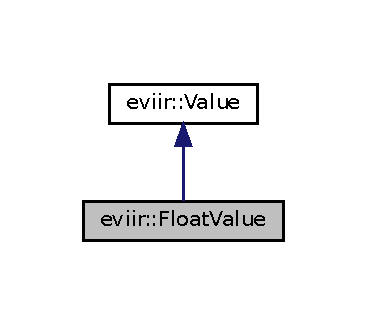
\includegraphics[width=180pt]{classeviir_1_1FloatValue__inherit__graph}
\end{center}
\end{figure}


Collaboration diagram for eviir\+:\+:Float\+Value\+:\nopagebreak
\begin{figure}[H]
\begin{center}
\leavevmode
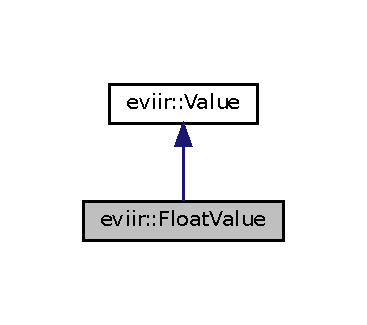
\includegraphics[width=180pt]{classeviir_1_1FloatValue__coll__graph}
\end{center}
\end{figure}
\subsection*{Public Member Functions}
\begin{DoxyCompactItemize}
\item 
string \hyperlink{classeviir_1_1FloatValue_a8713d6eb43445ba56c4104bce8fe7070}{generate\+\_\+ir} (const char $\ast$format=nullptr)
\item 
\mbox{\Hypertarget{classeviir_1_1FloatValue_a0ef754397965b49c1c547f476ae64bec}\label{classeviir_1_1FloatValue_a0ef754397965b49c1c547f476ae64bec}} 
{\bfseries Float\+Value} (float2 value)
\end{DoxyCompactItemize}
\subsection*{Public Attributes}
\begin{DoxyCompactItemize}
\item 
\mbox{\Hypertarget{classeviir_1_1FloatValue_a358648f87126c79adda8949f272fb56d}\label{classeviir_1_1FloatValue_a358648f87126c79adda8949f272fb56d}} 
float2 {\bfseries value}
\end{DoxyCompactItemize}
\subsection*{Additional Inherited Members}


\subsection{Member Function Documentation}
\mbox{\Hypertarget{classeviir_1_1FloatValue_a8713d6eb43445ba56c4104bce8fe7070}\label{classeviir_1_1FloatValue_a8713d6eb43445ba56c4104bce8fe7070}} 
\index{eviir\+::\+Float\+Value@{eviir\+::\+Float\+Value}!generate\+\_\+ir@{generate\+\_\+ir}}
\index{generate\+\_\+ir@{generate\+\_\+ir}!eviir\+::\+Float\+Value@{eviir\+::\+Float\+Value}}
\subsubsection{\texorpdfstring{generate\+\_\+ir()}{generate\_ir()}}
{\footnotesize\ttfamily string eviir\+::\+Float\+Value\+::generate\+\_\+ir (\begin{DoxyParamCaption}\item[{const char $\ast$}]{format = {\ttfamily nullptr} }\end{DoxyParamCaption})\hspace{0.3cm}{\ttfamily [virtual]}}

Generates the IR for the value \begin{DoxyReturn}{Returns}
the IR as a string (without newline) 
\end{DoxyReturn}


Implements \hyperlink{classeviir_1_1Value_a0613bf660425df31e230681555f64dea}{eviir\+::\+Value}.



The documentation for this class was generated from the following file\+:\begin{DoxyCompactItemize}
\item 
include/ir/value.\+hpp\end{DoxyCompactItemize}

\hypertarget{classeviir_1_1IntegerValue}{}\section{eviir\+:\+:Integer\+Value Class Reference}
\label{classeviir_1_1IntegerValue}\index{eviir\+::\+Integer\+Value@{eviir\+::\+Integer\+Value}}


Inheritance diagram for eviir\+:\+:Integer\+Value\+:\nopagebreak
\begin{figure}[H]
\begin{center}
\leavevmode
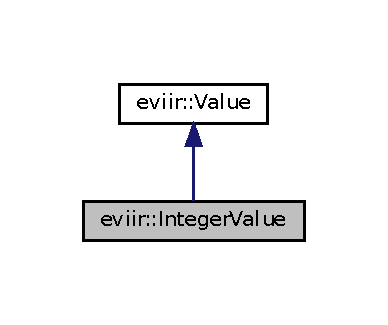
\includegraphics[width=192pt]{classeviir_1_1IntegerValue__inherit__graph}
\end{center}
\end{figure}


Collaboration diagram for eviir\+:\+:Integer\+Value\+:\nopagebreak
\begin{figure}[H]
\begin{center}
\leavevmode
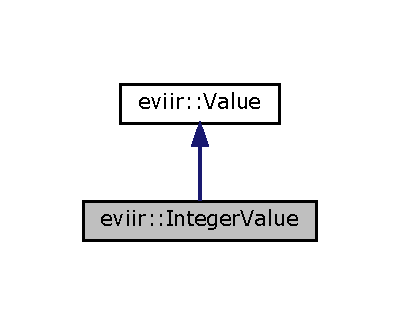
\includegraphics[width=192pt]{classeviir_1_1IntegerValue__coll__graph}
\end{center}
\end{figure}
\subsection*{Public Member Functions}
\begin{DoxyCompactItemize}
\item 
string \hyperlink{classeviir_1_1IntegerValue_a7f2653e23a8165a0eb43109d152cc0a2}{generate\+\_\+ir} (const char $\ast$format=nullptr)
\item 
\mbox{\Hypertarget{classeviir_1_1IntegerValue_a3820420d866c81f5bd8151a745ddaf8a}\label{classeviir_1_1IntegerValue_a3820420d866c81f5bd8151a745ddaf8a}} 
{\bfseries Integer\+Value} (int64 value)
\end{DoxyCompactItemize}
\subsection*{Public Attributes}
\begin{DoxyCompactItemize}
\item 
\mbox{\Hypertarget{classeviir_1_1IntegerValue_a6daae2d429977f76c8b1ab3b00a4ec33}\label{classeviir_1_1IntegerValue_a6daae2d429977f76c8b1ab3b00a4ec33}} 
int64 {\bfseries value}
\end{DoxyCompactItemize}


\subsection{Member Function Documentation}
\mbox{\Hypertarget{classeviir_1_1IntegerValue_a7f2653e23a8165a0eb43109d152cc0a2}\label{classeviir_1_1IntegerValue_a7f2653e23a8165a0eb43109d152cc0a2}} 
\index{eviir\+::\+Integer\+Value@{eviir\+::\+Integer\+Value}!generate\+\_\+ir@{generate\+\_\+ir}}
\index{generate\+\_\+ir@{generate\+\_\+ir}!eviir\+::\+Integer\+Value@{eviir\+::\+Integer\+Value}}
\subsubsection{\texorpdfstring{generate\+\_\+ir()}{generate\_ir()}}
{\footnotesize\ttfamily string eviir\+::\+Integer\+Value\+::generate\+\_\+ir (\begin{DoxyParamCaption}\item[{const char $\ast$}]{format = {\ttfamily nullptr} }\end{DoxyParamCaption})\hspace{0.3cm}{\ttfamily [virtual]}}

Generates the IR for the value \begin{DoxyReturn}{Returns}
the IR as a string (without newline) 
\end{DoxyReturn}


Implements \hyperlink{classeviir_1_1Value_a0613bf660425df31e230681555f64dea}{eviir\+::\+Value}.



The documentation for this class was generated from the following file\+:\begin{DoxyCompactItemize}
\item 
include/ir/value.\+hpp\end{DoxyCompactItemize}

\hypertarget{classeviir_1_1IRBuilder}{}\section{eviir\+:\+:I\+R\+Builder Class Reference}
\label{classeviir_1_1IRBuilder}\index{eviir\+::\+I\+R\+Builder@{eviir\+::\+I\+R\+Builder}}


A class for creating and managing instructions.  


\subsection*{Public Member Functions}
\begin{DoxyCompactItemize}
\item 
\mbox{\Hypertarget{classeviir_1_1IRBuilder_aaf6a6fb0af47e52dc6f2f16f90a7a62e}\label{classeviir_1_1IRBuilder_aaf6a6fb0af47e52dc6f2f16f90a7a62e}} 
\hyperlink{classeviir_1_1IRBuilder_aaf6a6fb0af47e52dc6f2f16f90a7a62e}{I\+R\+Builder} ()
\begin{DoxyCompactList}\small\item\em Constructs a new IR Builder. \end{DoxyCompactList}\end{DoxyCompactItemize}


\subsection{Detailed Description}
A class for creating and managing instructions. 

Instructions will be inserted in a \hyperlink{}{Basic\+Block}. ~\newline
Note that this A\+PI does not fully expose the uses of instructions. 

The documentation for this class was generated from the following file\+:\begin{DoxyCompactItemize}
\item 
include/ir/irbuilder.\+hpp\end{DoxyCompactItemize}

\hypertarget{classeviir_1_1ListValue}{}\doxysection{eviir\+::List\+Value Class Reference}
\label{classeviir_1_1ListValue}\index{eviir::ListValue@{eviir::ListValue}}


Inheritance diagram for eviir\+::List\+Value\+:
\nopagebreak
\begin{figure}[H]
\begin{center}
\leavevmode
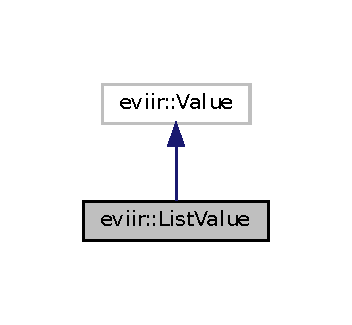
\includegraphics[width=169pt]{classeviir_1_1ListValue__inherit__graph}
\end{center}
\end{figure}


Collaboration diagram for eviir\+::List\+Value\+:
\nopagebreak
\begin{figure}[H]
\begin{center}
\leavevmode
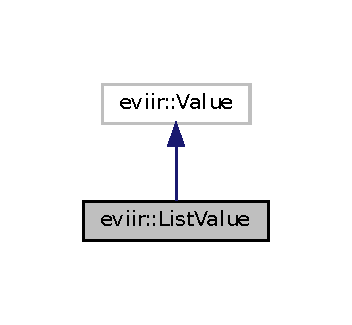
\includegraphics[width=169pt]{classeviir_1_1ListValue__coll__graph}
\end{center}
\end{figure}
\doxysubsection*{Public Member Functions}
\begin{DoxyCompactItemize}
\item 
string \mbox{\hyperlink{classeviir_1_1ListValue_ad12dee3774ad443ad0e27354909e8dc9}{generate\+\_\+ir}} (const char $\ast$format=nullptr)
\item 
\mbox{\Hypertarget{classeviir_1_1ListValue_ab6e8fba0e797ddafd95aef7763081505}\label{classeviir_1_1ListValue_ab6e8fba0e797ddafd95aef7763081505}} 
{\bfseries List\+Value} (vector$<$ \mbox{\hyperlink{classeviir_1_1Value}{Value}} $\ast$ $>$ elements)
\end{DoxyCompactItemize}
\doxysubsection*{Public Attributes}
\begin{DoxyCompactItemize}
\item 
\mbox{\Hypertarget{classeviir_1_1ListValue_a5bc8c31cf9ca0b62bc02edd6215c7612}\label{classeviir_1_1ListValue_a5bc8c31cf9ca0b62bc02edd6215c7612}} 
vector$<$ \mbox{\hyperlink{classeviir_1_1Value}{Value}} $\ast$ $>$ {\bfseries elements}
\end{DoxyCompactItemize}
\doxysubsection*{Additional Inherited Members}


\doxysubsection{Member Function Documentation}
\mbox{\Hypertarget{classeviir_1_1ListValue_ad12dee3774ad443ad0e27354909e8dc9}\label{classeviir_1_1ListValue_ad12dee3774ad443ad0e27354909e8dc9}} 
\index{eviir::ListValue@{eviir::ListValue}!generate\_ir@{generate\_ir}}
\index{generate\_ir@{generate\_ir}!eviir::ListValue@{eviir::ListValue}}
\doxysubsubsection{\texorpdfstring{generate\_ir()}{generate\_ir()}}
{\footnotesize\ttfamily string eviir\+::\+List\+Value\+::generate\+\_\+ir (\begin{DoxyParamCaption}\item[{const char $\ast$}]{format = {\ttfamily nullptr} }\end{DoxyParamCaption})\hspace{0.3cm}{\ttfamily [virtual]}}

Generates the IR for the value \begin{DoxyReturn}{Returns}
the IR as a string (without newline) 
\end{DoxyReturn}


Implements \mbox{\hyperlink{classeviir_1_1Value_a0613bf660425df31e230681555f64dea}{eviir\+::\+Value}}.



The documentation for this class was generated from the following file\+:\begin{DoxyCompactItemize}
\item 
/home/sjoerd/\+Coding/\+Languages/\+Evi\+Ir/include/ir/value.\+hpp\end{DoxyCompactItemize}

\hypertarget{classeviir_1_1Metadata}{}\section{eviir\+:\+:Metadata Class Reference}
\label{classeviir_1_1Metadata}\index{eviir\+::\+Metadata@{eviir\+::\+Metadata}}


A class defining the metadata of a \hyperlink{classeviir_1_1Module}{Module}.  


\subsection*{Public Types}
\begin{DoxyCompactItemize}
\item 
enum \hyperlink{classeviir_1_1Metadata_a372fe4af91ebc18a6d02354e8bcf23cf}{builtin\+\_\+property\+\_\+type} \{ \newline
\hyperlink{classeviir_1_1Metadata_a372fe4af91ebc18a6d02354e8bcf23cfab74b3d0d418e4382dc31e2ec0a971999}{M\+E\+T\+A\+\_\+\+M\+O\+D\+U\+L\+E\+\_\+\+N\+A\+ME}, 
\newline
\hyperlink{classeviir_1_1Metadata_a372fe4af91ebc18a6d02354e8bcf23cfabe2badced095f48ee8e7c2c7d67dd076}{M\+E\+T\+A\+\_\+\+M\+O\+D\+U\+L\+E\+\_\+\+E\+N\+T\+R\+Y\+P\+O\+I\+NT}, 
\newline
\hyperlink{classeviir_1_1Metadata_a372fe4af91ebc18a6d02354e8bcf23cfaa4c98efe507cf0505d60cdb343adf91d}{M\+E\+T\+A\+\_\+\+M\+O\+D\+U\+L\+E\+\_\+\+S\+O\+U\+R\+C\+E\+\_\+\+F\+I\+L\+E\+N\+A\+ME}, 
\newline
\hyperlink{classeviir_1_1Metadata_a372fe4af91ebc18a6d02354e8bcf23cfad817637faca96aa70195396a0c6c3c4e}{M\+E\+T\+A\+\_\+\+M\+O\+D\+U\+L\+E\+\_\+\+S\+O\+U\+R\+C\+E\+\_\+\+D\+I\+R\+E\+C\+T\+O\+RY}, 
\newline
\hyperlink{classeviir_1_1Metadata_a372fe4af91ebc18a6d02354e8bcf23cfacf7fdcaa5ed555d3d97fc79276417234}{M\+E\+T\+A\+\_\+\+M\+O\+D\+U\+L\+E\+\_\+\+S\+O\+U\+R\+C\+E\+\_\+\+L\+A\+N\+G\+U\+A\+GE}, 
\newline
\hyperlink{classeviir_1_1Metadata_a372fe4af91ebc18a6d02354e8bcf23cfaa665ac35c0944d7bccca7f7430b6947f}{M\+E\+T\+A\+\_\+\+M\+O\+D\+U\+L\+E\+\_\+\+P\+R\+O\+D\+U\+C\+E\+R\+\_\+\+N\+A\+ME}, 
\newline
\hyperlink{classeviir_1_1Metadata_a372fe4af91ebc18a6d02354e8bcf23cfac60c0ed594013e96d929a33813f62773}{M\+E\+T\+A\+\_\+\+M\+O\+D\+U\+L\+E\+\_\+\+P\+R\+O\+D\+U\+C\+E\+R\+\_\+\+V\+E\+R\+S\+I\+ON}, 
\newline
\hyperlink{classeviir_1_1Metadata_a372fe4af91ebc18a6d02354e8bcf23cfa92111e61fcb0fbda98d3da2d5e43017c}{M\+E\+T\+A\+\_\+\+M\+O\+D\+U\+L\+E\+\_\+\+P\+R\+O\+D\+U\+C\+E\+R\+\_\+\+T\+Y\+PE}, 
\newline
\hyperlink{classeviir_1_1Metadata_a372fe4af91ebc18a6d02354e8bcf23cfac19b0a19dd8bf62ea2590c1e66e2ad29}{M\+E\+T\+A\+\_\+\+T\+A\+R\+G\+E\+T\+\_\+\+T\+R\+I\+P\+LE}, 
\newline
\hyperlink{classeviir_1_1Metadata_a372fe4af91ebc18a6d02354e8bcf23cfa845ae2876378e855322c36ce699361d9}{M\+E\+T\+A\+\_\+\+T\+A\+R\+G\+E\+T\+\_\+\+C\+PU}, 
\newline
\hyperlink{classeviir_1_1Metadata_a372fe4af91ebc18a6d02354e8bcf23cfae559dded6278c6b59450355d624ed813}{M\+E\+T\+A\+\_\+\+T\+A\+R\+G\+E\+T\+\_\+\+D\+A\+T\+A\+L\+A\+Y\+O\+UT}, 
\newline
\hyperlink{classeviir_1_1Metadata_a372fe4af91ebc18a6d02354e8bcf23cfa30de1275b1bd0bbd22f4152125165d64}{M\+E\+T\+A\+\_\+\+T\+A\+R\+G\+E\+T\+\_\+\+O\+P\+T\+I\+M\+I\+Z\+A\+T\+I\+ON}, 
\newline
\hyperlink{classeviir_1_1Metadata_a372fe4af91ebc18a6d02354e8bcf23cfa56c810f16183314052f2835e34a6d4c0}{M\+E\+T\+A\+\_\+\+D\+E\+B\+U\+G\+\_\+\+G\+E\+N\+E\+R\+A\+TE}, 
\newline
\hyperlink{classeviir_1_1Metadata_a372fe4af91ebc18a6d02354e8bcf23cfad4a9ef6cce5a2a91449e2d55a9803f24}{M\+E\+T\+A\+\_\+\+D\+E\+B\+U\+G\+\_\+\+I\+N\+C\+L\+U\+D\+E\+S\+O\+U\+R\+CE}, 
\newline
\hyperlink{classeviir_1_1Metadata_a372fe4af91ebc18a6d02354e8bcf23cfaf7e6f8402e6d613f5f66f9dc01616476}{M\+E\+T\+A\+\_\+\+D\+E\+B\+U\+G\+\_\+\+S\+O\+U\+R\+C\+E\+L\+O\+C\+A\+T\+I\+ON}, 
\newline
\hyperlink{classeviir_1_1Metadata_a372fe4af91ebc18a6d02354e8bcf23cfabc019a6c020745255aec2bc76c4b88b6}{M\+E\+T\+A\+\_\+\+D\+E\+B\+U\+G\+\_\+\+S\+O\+U\+R\+C\+E\+C\+H\+E\+C\+K\+S\+UM}, 
\newline
\hyperlink{classeviir_1_1Metadata_a372fe4af91ebc18a6d02354e8bcf23cfa29269f7064f3dd0aa1875f810931ce35}{M\+E\+T\+A\+\_\+\+D\+E\+B\+U\+G\+\_\+\+D\+W\+A\+R\+F\+V\+E\+R\+S\+I\+ON}, 
\newline
\hyperlink{classeviir_1_1Metadata_a372fe4af91ebc18a6d02354e8bcf23cfaaf03cdca11331e82463a7168a9dca2e5}{M\+E\+T\+A\+\_\+\+D\+E\+B\+U\+G\+\_\+\+T\+Y\+P\+E\+N\+A\+M\+ES}
 \}\begin{DoxyCompactList}\small\item\em built-\/in metadata property types. \end{DoxyCompactList}
\item 
enum \hyperlink{classeviir_1_1Metadata_a890ce3566bd1dc49d5b1da4abb9b8490}{custom\+\_\+property\+\_\+type} \{ \newline
\hyperlink{classeviir_1_1Metadata_a890ce3566bd1dc49d5b1da4abb9b8490ad189e84d060c629c555c0d875e26e7f5}{M\+E\+T\+A\+\_\+\+M\+O\+D\+U\+LE}, 
\newline
\hyperlink{classeviir_1_1Metadata_a890ce3566bd1dc49d5b1da4abb9b8490a4cf1ed5320fab8b379cab80128a5f947}{M\+E\+T\+A\+\_\+\+M\+O\+D\+U\+L\+E\+\_\+\+S\+O\+U\+R\+CE}, 
\newline
\hyperlink{classeviir_1_1Metadata_a890ce3566bd1dc49d5b1da4abb9b8490a01b5801c88ba15043f5fc1dacab08cab}{M\+E\+T\+A\+\_\+\+M\+O\+D\+U\+L\+E\+\_\+\+P\+R\+O\+D\+U\+C\+ER}, 
\newline
\hyperlink{classeviir_1_1Metadata_a890ce3566bd1dc49d5b1da4abb9b8490ab27ef44c17f2098f805f27a2336e7e14}{M\+E\+T\+A\+\_\+\+T\+A\+R\+G\+ET}, 
\newline
\hyperlink{classeviir_1_1Metadata_a890ce3566bd1dc49d5b1da4abb9b8490a6cf8530b9dac75b50afc0621ce40a9c8}{M\+E\+T\+A\+\_\+\+D\+E\+B\+UG}, 
\newline
\hyperlink{classeviir_1_1Metadata_a890ce3566bd1dc49d5b1da4abb9b8490a75edc14cde2b7b26bb6d760fc9ee756d}{M\+E\+T\+A\+\_\+\+C\+U\+S\+T\+OM}
 \}\begin{DoxyCompactList}\small\item\em custom metadata property types. \end{DoxyCompactList}
\item 
\mbox{\Hypertarget{classeviir_1_1Metadata_ac613e5de0552301f9b7969d14eb5dffa}\label{classeviir_1_1Metadata_ac613e5de0552301f9b7969d14eb5dffa}} 
typedef vector$<$ string $>$ \hyperlink{classeviir_1_1Metadata_ac613e5de0552301f9b7969d14eb5dffa}{path}
\begin{DoxyCompactList}\small\item\em A metadata path. \end{DoxyCompactList}\end{DoxyCompactItemize}
\subsection*{Public Member Functions}
\begin{DoxyCompactItemize}
\item 
\hyperlink{classeviir_1_1Metadata_a932b55404878eeef14ad7d4e7ed98f9e}{Metadata} (\hyperlink{classeviir_1_1Metadata_a372fe4af91ebc18a6d02354e8bcf23cf}{builtin\+\_\+property\+\_\+type} type, \hyperlink{classeviir_1_1Value}{Value} $\ast$value=nullptr)
\item 
\hyperlink{classeviir_1_1Metadata_afd2f484427fcdf9aa777d6471251b3ea}{Metadata} (\hyperlink{classeviir_1_1Metadata_a890ce3566bd1dc49d5b1da4abb9b8490}{custom\+\_\+property\+\_\+type} type, \hyperlink{classeviir_1_1Metadata_ac613e5de0552301f9b7969d14eb5dffa}{path} \hyperlink{classeviir_1_1Metadata_ac613e5de0552301f9b7969d14eb5dffa}{path}, \hyperlink{classeviir_1_1Value}{Value} $\ast$value=nullptr)
\item 
string \hyperlink{classeviir_1_1Metadata_ab4ac3feef2692e4ae984842224787934}{generate\+\_\+ir} ()
\end{DoxyCompactItemize}
\subsection*{Static Public Member Functions}
\begin{DoxyCompactItemize}
\item 
static \hyperlink{classeviir_1_1Metadata_ac613e5de0552301f9b7969d14eb5dffa}{path} \hyperlink{classeviir_1_1Metadata_a39b71a74731f3357b5f0888c6b3ba3e4}{create\+\_\+path} (string full\+\_\+path)
\begin{DoxyCompactList}\small\item\em Creates a Metadata path. \end{DoxyCompactList}\end{DoxyCompactItemize}
\subsection*{Friends}
\begin{DoxyCompactItemize}
\item 
\mbox{\Hypertarget{classeviir_1_1Metadata_a21f639900c480510650969df9c74d17d}\label{classeviir_1_1Metadata_a21f639900c480510650969df9c74d17d}} 
class {\bfseries Module}
\end{DoxyCompactItemize}


\subsection{Detailed Description}
A class defining the metadata of a \hyperlink{classeviir_1_1Module}{Module}. 

Can be added to a module using \hyperlink{classeviir_1_1Module_a9e4bc38ac7d619c039a0bb0559589399}{Module\+::add\+\_\+metadata}. 

\subsection{Member Enumeration Documentation}
\mbox{\Hypertarget{classeviir_1_1Metadata_a372fe4af91ebc18a6d02354e8bcf23cf}\label{classeviir_1_1Metadata_a372fe4af91ebc18a6d02354e8bcf23cf}} 
\index{eviir\+::\+Metadata@{eviir\+::\+Metadata}!builtin\+\_\+property\+\_\+type@{builtin\+\_\+property\+\_\+type}}
\index{builtin\+\_\+property\+\_\+type@{builtin\+\_\+property\+\_\+type}!eviir\+::\+Metadata@{eviir\+::\+Metadata}}
\subsubsection{\texorpdfstring{builtin\+\_\+property\+\_\+type}{builtin\_property\_type}}
{\footnotesize\ttfamily enum \hyperlink{classeviir_1_1Metadata_a372fe4af91ebc18a6d02354e8bcf23cf}{eviir\+::\+Metadata\+::builtin\+\_\+property\+\_\+type}}



built-\/in metadata property types. 

Used by \hyperlink{}{Metadata\+::(builtin\+\_\+property\+\_\+type type, Value$\ast$ value = nullptr)}. \begin{DoxyEnumFields}{Enumerator}
\raisebox{\heightof{T}}[0pt][0pt]{\index{M\+E\+T\+A\+\_\+\+M\+O\+D\+U\+L\+E\+\_\+\+N\+A\+ME@{M\+E\+T\+A\+\_\+\+M\+O\+D\+U\+L\+E\+\_\+\+N\+A\+ME}!eviir\+::\+Metadata@{eviir\+::\+Metadata}}\index{eviir\+::\+Metadata@{eviir\+::\+Metadata}!M\+E\+T\+A\+\_\+\+M\+O\+D\+U\+L\+E\+\_\+\+N\+A\+ME@{M\+E\+T\+A\+\_\+\+M\+O\+D\+U\+L\+E\+\_\+\+N\+A\+ME}}}\mbox{\Hypertarget{classeviir_1_1Metadata_a372fe4af91ebc18a6d02354e8bcf23cfab74b3d0d418e4382dc31e2ec0a971999}\label{classeviir_1_1Metadata_a372fe4af91ebc18a6d02354e8bcf23cfab74b3d0d418e4382dc31e2ec0a971999}} 
M\+E\+T\+A\+\_\+\+M\+O\+D\+U\+L\+E\+\_\+\+N\+A\+ME&metadata property path\+: {\ttfamily !module/name} \\
\hline

\raisebox{\heightof{T}}[0pt][0pt]{\index{M\+E\+T\+A\+\_\+\+M\+O\+D\+U\+L\+E\+\_\+\+E\+N\+T\+R\+Y\+P\+O\+I\+NT@{M\+E\+T\+A\+\_\+\+M\+O\+D\+U\+L\+E\+\_\+\+E\+N\+T\+R\+Y\+P\+O\+I\+NT}!eviir\+::\+Metadata@{eviir\+::\+Metadata}}\index{eviir\+::\+Metadata@{eviir\+::\+Metadata}!M\+E\+T\+A\+\_\+\+M\+O\+D\+U\+L\+E\+\_\+\+E\+N\+T\+R\+Y\+P\+O\+I\+NT@{M\+E\+T\+A\+\_\+\+M\+O\+D\+U\+L\+E\+\_\+\+E\+N\+T\+R\+Y\+P\+O\+I\+NT}}}\mbox{\Hypertarget{classeviir_1_1Metadata_a372fe4af91ebc18a6d02354e8bcf23cfabe2badced095f48ee8e7c2c7d67dd076}\label{classeviir_1_1Metadata_a372fe4af91ebc18a6d02354e8bcf23cfabe2badced095f48ee8e7c2c7d67dd076}} 
M\+E\+T\+A\+\_\+\+M\+O\+D\+U\+L\+E\+\_\+\+E\+N\+T\+R\+Y\+P\+O\+I\+NT&metadata property path\+: {\ttfamily !module/entrypoint} \\
\hline

\raisebox{\heightof{T}}[0pt][0pt]{\index{M\+E\+T\+A\+\_\+\+M\+O\+D\+U\+L\+E\+\_\+\+S\+O\+U\+R\+C\+E\+\_\+\+F\+I\+L\+E\+N\+A\+ME@{M\+E\+T\+A\+\_\+\+M\+O\+D\+U\+L\+E\+\_\+\+S\+O\+U\+R\+C\+E\+\_\+\+F\+I\+L\+E\+N\+A\+ME}!eviir\+::\+Metadata@{eviir\+::\+Metadata}}\index{eviir\+::\+Metadata@{eviir\+::\+Metadata}!M\+E\+T\+A\+\_\+\+M\+O\+D\+U\+L\+E\+\_\+\+S\+O\+U\+R\+C\+E\+\_\+\+F\+I\+L\+E\+N\+A\+ME@{M\+E\+T\+A\+\_\+\+M\+O\+D\+U\+L\+E\+\_\+\+S\+O\+U\+R\+C\+E\+\_\+\+F\+I\+L\+E\+N\+A\+ME}}}\mbox{\Hypertarget{classeviir_1_1Metadata_a372fe4af91ebc18a6d02354e8bcf23cfaa4c98efe507cf0505d60cdb343adf91d}\label{classeviir_1_1Metadata_a372fe4af91ebc18a6d02354e8bcf23cfaa4c98efe507cf0505d60cdb343adf91d}} 
M\+E\+T\+A\+\_\+\+M\+O\+D\+U\+L\+E\+\_\+\+S\+O\+U\+R\+C\+E\+\_\+\+F\+I\+L\+E\+N\+A\+ME&metadata property path\+: {\ttfamily !module/source/filename} \\
\hline

\raisebox{\heightof{T}}[0pt][0pt]{\index{M\+E\+T\+A\+\_\+\+M\+O\+D\+U\+L\+E\+\_\+\+S\+O\+U\+R\+C\+E\+\_\+\+D\+I\+R\+E\+C\+T\+O\+RY@{M\+E\+T\+A\+\_\+\+M\+O\+D\+U\+L\+E\+\_\+\+S\+O\+U\+R\+C\+E\+\_\+\+D\+I\+R\+E\+C\+T\+O\+RY}!eviir\+::\+Metadata@{eviir\+::\+Metadata}}\index{eviir\+::\+Metadata@{eviir\+::\+Metadata}!M\+E\+T\+A\+\_\+\+M\+O\+D\+U\+L\+E\+\_\+\+S\+O\+U\+R\+C\+E\+\_\+\+D\+I\+R\+E\+C\+T\+O\+RY@{M\+E\+T\+A\+\_\+\+M\+O\+D\+U\+L\+E\+\_\+\+S\+O\+U\+R\+C\+E\+\_\+\+D\+I\+R\+E\+C\+T\+O\+RY}}}\mbox{\Hypertarget{classeviir_1_1Metadata_a372fe4af91ebc18a6d02354e8bcf23cfad817637faca96aa70195396a0c6c3c4e}\label{classeviir_1_1Metadata_a372fe4af91ebc18a6d02354e8bcf23cfad817637faca96aa70195396a0c6c3c4e}} 
M\+E\+T\+A\+\_\+\+M\+O\+D\+U\+L\+E\+\_\+\+S\+O\+U\+R\+C\+E\+\_\+\+D\+I\+R\+E\+C\+T\+O\+RY&metadata property path\+: {\ttfamily !module/source/directory} \\
\hline

\raisebox{\heightof{T}}[0pt][0pt]{\index{M\+E\+T\+A\+\_\+\+M\+O\+D\+U\+L\+E\+\_\+\+S\+O\+U\+R\+C\+E\+\_\+\+L\+A\+N\+G\+U\+A\+GE@{M\+E\+T\+A\+\_\+\+M\+O\+D\+U\+L\+E\+\_\+\+S\+O\+U\+R\+C\+E\+\_\+\+L\+A\+N\+G\+U\+A\+GE}!eviir\+::\+Metadata@{eviir\+::\+Metadata}}\index{eviir\+::\+Metadata@{eviir\+::\+Metadata}!M\+E\+T\+A\+\_\+\+M\+O\+D\+U\+L\+E\+\_\+\+S\+O\+U\+R\+C\+E\+\_\+\+L\+A\+N\+G\+U\+A\+GE@{M\+E\+T\+A\+\_\+\+M\+O\+D\+U\+L\+E\+\_\+\+S\+O\+U\+R\+C\+E\+\_\+\+L\+A\+N\+G\+U\+A\+GE}}}\mbox{\Hypertarget{classeviir_1_1Metadata_a372fe4af91ebc18a6d02354e8bcf23cfacf7fdcaa5ed555d3d97fc79276417234}\label{classeviir_1_1Metadata_a372fe4af91ebc18a6d02354e8bcf23cfacf7fdcaa5ed555d3d97fc79276417234}} 
M\+E\+T\+A\+\_\+\+M\+O\+D\+U\+L\+E\+\_\+\+S\+O\+U\+R\+C\+E\+\_\+\+L\+A\+N\+G\+U\+A\+GE&metadata property path\+: {\ttfamily !module/source/language} \\
\hline

\raisebox{\heightof{T}}[0pt][0pt]{\index{M\+E\+T\+A\+\_\+\+M\+O\+D\+U\+L\+E\+\_\+\+P\+R\+O\+D\+U\+C\+E\+R\+\_\+\+N\+A\+ME@{M\+E\+T\+A\+\_\+\+M\+O\+D\+U\+L\+E\+\_\+\+P\+R\+O\+D\+U\+C\+E\+R\+\_\+\+N\+A\+ME}!eviir\+::\+Metadata@{eviir\+::\+Metadata}}\index{eviir\+::\+Metadata@{eviir\+::\+Metadata}!M\+E\+T\+A\+\_\+\+M\+O\+D\+U\+L\+E\+\_\+\+P\+R\+O\+D\+U\+C\+E\+R\+\_\+\+N\+A\+ME@{M\+E\+T\+A\+\_\+\+M\+O\+D\+U\+L\+E\+\_\+\+P\+R\+O\+D\+U\+C\+E\+R\+\_\+\+N\+A\+ME}}}\mbox{\Hypertarget{classeviir_1_1Metadata_a372fe4af91ebc18a6d02354e8bcf23cfaa665ac35c0944d7bccca7f7430b6947f}\label{classeviir_1_1Metadata_a372fe4af91ebc18a6d02354e8bcf23cfaa665ac35c0944d7bccca7f7430b6947f}} 
M\+E\+T\+A\+\_\+\+M\+O\+D\+U\+L\+E\+\_\+\+P\+R\+O\+D\+U\+C\+E\+R\+\_\+\+N\+A\+ME&metadata property path\+: {\ttfamily !module/producer/name} \\
\hline

\raisebox{\heightof{T}}[0pt][0pt]{\index{M\+E\+T\+A\+\_\+\+M\+O\+D\+U\+L\+E\+\_\+\+P\+R\+O\+D\+U\+C\+E\+R\+\_\+\+V\+E\+R\+S\+I\+ON@{M\+E\+T\+A\+\_\+\+M\+O\+D\+U\+L\+E\+\_\+\+P\+R\+O\+D\+U\+C\+E\+R\+\_\+\+V\+E\+R\+S\+I\+ON}!eviir\+::\+Metadata@{eviir\+::\+Metadata}}\index{eviir\+::\+Metadata@{eviir\+::\+Metadata}!M\+E\+T\+A\+\_\+\+M\+O\+D\+U\+L\+E\+\_\+\+P\+R\+O\+D\+U\+C\+E\+R\+\_\+\+V\+E\+R\+S\+I\+ON@{M\+E\+T\+A\+\_\+\+M\+O\+D\+U\+L\+E\+\_\+\+P\+R\+O\+D\+U\+C\+E\+R\+\_\+\+V\+E\+R\+S\+I\+ON}}}\mbox{\Hypertarget{classeviir_1_1Metadata_a372fe4af91ebc18a6d02354e8bcf23cfac60c0ed594013e96d929a33813f62773}\label{classeviir_1_1Metadata_a372fe4af91ebc18a6d02354e8bcf23cfac60c0ed594013e96d929a33813f62773}} 
M\+E\+T\+A\+\_\+\+M\+O\+D\+U\+L\+E\+\_\+\+P\+R\+O\+D\+U\+C\+E\+R\+\_\+\+V\+E\+R\+S\+I\+ON&metadata property path\+: {\ttfamily !module/producer/version} \\
\hline

\raisebox{\heightof{T}}[0pt][0pt]{\index{M\+E\+T\+A\+\_\+\+M\+O\+D\+U\+L\+E\+\_\+\+P\+R\+O\+D\+U\+C\+E\+R\+\_\+\+T\+Y\+PE@{M\+E\+T\+A\+\_\+\+M\+O\+D\+U\+L\+E\+\_\+\+P\+R\+O\+D\+U\+C\+E\+R\+\_\+\+T\+Y\+PE}!eviir\+::\+Metadata@{eviir\+::\+Metadata}}\index{eviir\+::\+Metadata@{eviir\+::\+Metadata}!M\+E\+T\+A\+\_\+\+M\+O\+D\+U\+L\+E\+\_\+\+P\+R\+O\+D\+U\+C\+E\+R\+\_\+\+T\+Y\+PE@{M\+E\+T\+A\+\_\+\+M\+O\+D\+U\+L\+E\+\_\+\+P\+R\+O\+D\+U\+C\+E\+R\+\_\+\+T\+Y\+PE}}}\mbox{\Hypertarget{classeviir_1_1Metadata_a372fe4af91ebc18a6d02354e8bcf23cfa92111e61fcb0fbda98d3da2d5e43017c}\label{classeviir_1_1Metadata_a372fe4af91ebc18a6d02354e8bcf23cfa92111e61fcb0fbda98d3da2d5e43017c}} 
M\+E\+T\+A\+\_\+\+M\+O\+D\+U\+L\+E\+\_\+\+P\+R\+O\+D\+U\+C\+E\+R\+\_\+\+T\+Y\+PE&metadata property path\+: {\ttfamily !module/producer/type} \\
\hline

\raisebox{\heightof{T}}[0pt][0pt]{\index{M\+E\+T\+A\+\_\+\+T\+A\+R\+G\+E\+T\+\_\+\+T\+R\+I\+P\+LE@{M\+E\+T\+A\+\_\+\+T\+A\+R\+G\+E\+T\+\_\+\+T\+R\+I\+P\+LE}!eviir\+::\+Metadata@{eviir\+::\+Metadata}}\index{eviir\+::\+Metadata@{eviir\+::\+Metadata}!M\+E\+T\+A\+\_\+\+T\+A\+R\+G\+E\+T\+\_\+\+T\+R\+I\+P\+LE@{M\+E\+T\+A\+\_\+\+T\+A\+R\+G\+E\+T\+\_\+\+T\+R\+I\+P\+LE}}}\mbox{\Hypertarget{classeviir_1_1Metadata_a372fe4af91ebc18a6d02354e8bcf23cfac19b0a19dd8bf62ea2590c1e66e2ad29}\label{classeviir_1_1Metadata_a372fe4af91ebc18a6d02354e8bcf23cfac19b0a19dd8bf62ea2590c1e66e2ad29}} 
M\+E\+T\+A\+\_\+\+T\+A\+R\+G\+E\+T\+\_\+\+T\+R\+I\+P\+LE&metadata property path\+: {\ttfamily !target/triple} \\
\hline

\raisebox{\heightof{T}}[0pt][0pt]{\index{M\+E\+T\+A\+\_\+\+T\+A\+R\+G\+E\+T\+\_\+\+C\+PU@{M\+E\+T\+A\+\_\+\+T\+A\+R\+G\+E\+T\+\_\+\+C\+PU}!eviir\+::\+Metadata@{eviir\+::\+Metadata}}\index{eviir\+::\+Metadata@{eviir\+::\+Metadata}!M\+E\+T\+A\+\_\+\+T\+A\+R\+G\+E\+T\+\_\+\+C\+PU@{M\+E\+T\+A\+\_\+\+T\+A\+R\+G\+E\+T\+\_\+\+C\+PU}}}\mbox{\Hypertarget{classeviir_1_1Metadata_a372fe4af91ebc18a6d02354e8bcf23cfa845ae2876378e855322c36ce699361d9}\label{classeviir_1_1Metadata_a372fe4af91ebc18a6d02354e8bcf23cfa845ae2876378e855322c36ce699361d9}} 
M\+E\+T\+A\+\_\+\+T\+A\+R\+G\+E\+T\+\_\+\+C\+PU&metadata property path\+: {\ttfamily !target/cpu} \\
\hline

\raisebox{\heightof{T}}[0pt][0pt]{\index{M\+E\+T\+A\+\_\+\+T\+A\+R\+G\+E\+T\+\_\+\+D\+A\+T\+A\+L\+A\+Y\+O\+UT@{M\+E\+T\+A\+\_\+\+T\+A\+R\+G\+E\+T\+\_\+\+D\+A\+T\+A\+L\+A\+Y\+O\+UT}!eviir\+::\+Metadata@{eviir\+::\+Metadata}}\index{eviir\+::\+Metadata@{eviir\+::\+Metadata}!M\+E\+T\+A\+\_\+\+T\+A\+R\+G\+E\+T\+\_\+\+D\+A\+T\+A\+L\+A\+Y\+O\+UT@{M\+E\+T\+A\+\_\+\+T\+A\+R\+G\+E\+T\+\_\+\+D\+A\+T\+A\+L\+A\+Y\+O\+UT}}}\mbox{\Hypertarget{classeviir_1_1Metadata_a372fe4af91ebc18a6d02354e8bcf23cfae559dded6278c6b59450355d624ed813}\label{classeviir_1_1Metadata_a372fe4af91ebc18a6d02354e8bcf23cfae559dded6278c6b59450355d624ed813}} 
M\+E\+T\+A\+\_\+\+T\+A\+R\+G\+E\+T\+\_\+\+D\+A\+T\+A\+L\+A\+Y\+O\+UT&metadata property path\+: {\ttfamily !target/datalayout} \\
\hline

\raisebox{\heightof{T}}[0pt][0pt]{\index{M\+E\+T\+A\+\_\+\+T\+A\+R\+G\+E\+T\+\_\+\+O\+P\+T\+I\+M\+I\+Z\+A\+T\+I\+ON@{M\+E\+T\+A\+\_\+\+T\+A\+R\+G\+E\+T\+\_\+\+O\+P\+T\+I\+M\+I\+Z\+A\+T\+I\+ON}!eviir\+::\+Metadata@{eviir\+::\+Metadata}}\index{eviir\+::\+Metadata@{eviir\+::\+Metadata}!M\+E\+T\+A\+\_\+\+T\+A\+R\+G\+E\+T\+\_\+\+O\+P\+T\+I\+M\+I\+Z\+A\+T\+I\+ON@{M\+E\+T\+A\+\_\+\+T\+A\+R\+G\+E\+T\+\_\+\+O\+P\+T\+I\+M\+I\+Z\+A\+T\+I\+ON}}}\mbox{\Hypertarget{classeviir_1_1Metadata_a372fe4af91ebc18a6d02354e8bcf23cfa30de1275b1bd0bbd22f4152125165d64}\label{classeviir_1_1Metadata_a372fe4af91ebc18a6d02354e8bcf23cfa30de1275b1bd0bbd22f4152125165d64}} 
M\+E\+T\+A\+\_\+\+T\+A\+R\+G\+E\+T\+\_\+\+O\+P\+T\+I\+M\+I\+Z\+A\+T\+I\+ON&metadata property path\+: {\ttfamily !target/optimization} \\
\hline

\raisebox{\heightof{T}}[0pt][0pt]{\index{M\+E\+T\+A\+\_\+\+D\+E\+B\+U\+G\+\_\+\+G\+E\+N\+E\+R\+A\+TE@{M\+E\+T\+A\+\_\+\+D\+E\+B\+U\+G\+\_\+\+G\+E\+N\+E\+R\+A\+TE}!eviir\+::\+Metadata@{eviir\+::\+Metadata}}\index{eviir\+::\+Metadata@{eviir\+::\+Metadata}!M\+E\+T\+A\+\_\+\+D\+E\+B\+U\+G\+\_\+\+G\+E\+N\+E\+R\+A\+TE@{M\+E\+T\+A\+\_\+\+D\+E\+B\+U\+G\+\_\+\+G\+E\+N\+E\+R\+A\+TE}}}\mbox{\Hypertarget{classeviir_1_1Metadata_a372fe4af91ebc18a6d02354e8bcf23cfa56c810f16183314052f2835e34a6d4c0}\label{classeviir_1_1Metadata_a372fe4af91ebc18a6d02354e8bcf23cfa56c810f16183314052f2835e34a6d4c0}} 
M\+E\+T\+A\+\_\+\+D\+E\+B\+U\+G\+\_\+\+G\+E\+N\+E\+R\+A\+TE&metadata property path\+: {\ttfamily !debug/generate} \\
\hline

\raisebox{\heightof{T}}[0pt][0pt]{\index{M\+E\+T\+A\+\_\+\+D\+E\+B\+U\+G\+\_\+\+I\+N\+C\+L\+U\+D\+E\+S\+O\+U\+R\+CE@{M\+E\+T\+A\+\_\+\+D\+E\+B\+U\+G\+\_\+\+I\+N\+C\+L\+U\+D\+E\+S\+O\+U\+R\+CE}!eviir\+::\+Metadata@{eviir\+::\+Metadata}}\index{eviir\+::\+Metadata@{eviir\+::\+Metadata}!M\+E\+T\+A\+\_\+\+D\+E\+B\+U\+G\+\_\+\+I\+N\+C\+L\+U\+D\+E\+S\+O\+U\+R\+CE@{M\+E\+T\+A\+\_\+\+D\+E\+B\+U\+G\+\_\+\+I\+N\+C\+L\+U\+D\+E\+S\+O\+U\+R\+CE}}}\mbox{\Hypertarget{classeviir_1_1Metadata_a372fe4af91ebc18a6d02354e8bcf23cfad4a9ef6cce5a2a91449e2d55a9803f24}\label{classeviir_1_1Metadata_a372fe4af91ebc18a6d02354e8bcf23cfad4a9ef6cce5a2a91449e2d55a9803f24}} 
M\+E\+T\+A\+\_\+\+D\+E\+B\+U\+G\+\_\+\+I\+N\+C\+L\+U\+D\+E\+S\+O\+U\+R\+CE&metadata property path\+: {\ttfamily !debug/includesource} \\
\hline

\raisebox{\heightof{T}}[0pt][0pt]{\index{M\+E\+T\+A\+\_\+\+D\+E\+B\+U\+G\+\_\+\+S\+O\+U\+R\+C\+E\+L\+O\+C\+A\+T\+I\+ON@{M\+E\+T\+A\+\_\+\+D\+E\+B\+U\+G\+\_\+\+S\+O\+U\+R\+C\+E\+L\+O\+C\+A\+T\+I\+ON}!eviir\+::\+Metadata@{eviir\+::\+Metadata}}\index{eviir\+::\+Metadata@{eviir\+::\+Metadata}!M\+E\+T\+A\+\_\+\+D\+E\+B\+U\+G\+\_\+\+S\+O\+U\+R\+C\+E\+L\+O\+C\+A\+T\+I\+ON@{M\+E\+T\+A\+\_\+\+D\+E\+B\+U\+G\+\_\+\+S\+O\+U\+R\+C\+E\+L\+O\+C\+A\+T\+I\+ON}}}\mbox{\Hypertarget{classeviir_1_1Metadata_a372fe4af91ebc18a6d02354e8bcf23cfaf7e6f8402e6d613f5f66f9dc01616476}\label{classeviir_1_1Metadata_a372fe4af91ebc18a6d02354e8bcf23cfaf7e6f8402e6d613f5f66f9dc01616476}} 
M\+E\+T\+A\+\_\+\+D\+E\+B\+U\+G\+\_\+\+S\+O\+U\+R\+C\+E\+L\+O\+C\+A\+T\+I\+ON&metadata property path\+: {\ttfamily !debug/sourcelocation} \\
\hline

\raisebox{\heightof{T}}[0pt][0pt]{\index{M\+E\+T\+A\+\_\+\+D\+E\+B\+U\+G\+\_\+\+S\+O\+U\+R\+C\+E\+C\+H\+E\+C\+K\+S\+UM@{M\+E\+T\+A\+\_\+\+D\+E\+B\+U\+G\+\_\+\+S\+O\+U\+R\+C\+E\+C\+H\+E\+C\+K\+S\+UM}!eviir\+::\+Metadata@{eviir\+::\+Metadata}}\index{eviir\+::\+Metadata@{eviir\+::\+Metadata}!M\+E\+T\+A\+\_\+\+D\+E\+B\+U\+G\+\_\+\+S\+O\+U\+R\+C\+E\+C\+H\+E\+C\+K\+S\+UM@{M\+E\+T\+A\+\_\+\+D\+E\+B\+U\+G\+\_\+\+S\+O\+U\+R\+C\+E\+C\+H\+E\+C\+K\+S\+UM}}}\mbox{\Hypertarget{classeviir_1_1Metadata_a372fe4af91ebc18a6d02354e8bcf23cfabc019a6c020745255aec2bc76c4b88b6}\label{classeviir_1_1Metadata_a372fe4af91ebc18a6d02354e8bcf23cfabc019a6c020745255aec2bc76c4b88b6}} 
M\+E\+T\+A\+\_\+\+D\+E\+B\+U\+G\+\_\+\+S\+O\+U\+R\+C\+E\+C\+H\+E\+C\+K\+S\+UM&metadata property path\+: {\ttfamily !debug/sourcechecksum} \\
\hline

\raisebox{\heightof{T}}[0pt][0pt]{\index{M\+E\+T\+A\+\_\+\+D\+E\+B\+U\+G\+\_\+\+D\+W\+A\+R\+F\+V\+E\+R\+S\+I\+ON@{M\+E\+T\+A\+\_\+\+D\+E\+B\+U\+G\+\_\+\+D\+W\+A\+R\+F\+V\+E\+R\+S\+I\+ON}!eviir\+::\+Metadata@{eviir\+::\+Metadata}}\index{eviir\+::\+Metadata@{eviir\+::\+Metadata}!M\+E\+T\+A\+\_\+\+D\+E\+B\+U\+G\+\_\+\+D\+W\+A\+R\+F\+V\+E\+R\+S\+I\+ON@{M\+E\+T\+A\+\_\+\+D\+E\+B\+U\+G\+\_\+\+D\+W\+A\+R\+F\+V\+E\+R\+S\+I\+ON}}}\mbox{\Hypertarget{classeviir_1_1Metadata_a372fe4af91ebc18a6d02354e8bcf23cfa29269f7064f3dd0aa1875f810931ce35}\label{classeviir_1_1Metadata_a372fe4af91ebc18a6d02354e8bcf23cfa29269f7064f3dd0aa1875f810931ce35}} 
M\+E\+T\+A\+\_\+\+D\+E\+B\+U\+G\+\_\+\+D\+W\+A\+R\+F\+V\+E\+R\+S\+I\+ON&metadata property path\+: {\ttfamily !debug/dwarfversion} \\
\hline

\raisebox{\heightof{T}}[0pt][0pt]{\index{M\+E\+T\+A\+\_\+\+D\+E\+B\+U\+G\+\_\+\+T\+Y\+P\+E\+N\+A\+M\+ES@{M\+E\+T\+A\+\_\+\+D\+E\+B\+U\+G\+\_\+\+T\+Y\+P\+E\+N\+A\+M\+ES}!eviir\+::\+Metadata@{eviir\+::\+Metadata}}\index{eviir\+::\+Metadata@{eviir\+::\+Metadata}!M\+E\+T\+A\+\_\+\+D\+E\+B\+U\+G\+\_\+\+T\+Y\+P\+E\+N\+A\+M\+ES@{M\+E\+T\+A\+\_\+\+D\+E\+B\+U\+G\+\_\+\+T\+Y\+P\+E\+N\+A\+M\+ES}}}\mbox{\Hypertarget{classeviir_1_1Metadata_a372fe4af91ebc18a6d02354e8bcf23cfaaf03cdca11331e82463a7168a9dca2e5}\label{classeviir_1_1Metadata_a372fe4af91ebc18a6d02354e8bcf23cfaaf03cdca11331e82463a7168a9dca2e5}} 
M\+E\+T\+A\+\_\+\+D\+E\+B\+U\+G\+\_\+\+T\+Y\+P\+E\+N\+A\+M\+ES&metadata property path\+: {\ttfamily !debug/typenames} \\
\hline

\end{DoxyEnumFields}
\mbox{\Hypertarget{classeviir_1_1Metadata_a890ce3566bd1dc49d5b1da4abb9b8490}\label{classeviir_1_1Metadata_a890ce3566bd1dc49d5b1da4abb9b8490}} 
\index{eviir\+::\+Metadata@{eviir\+::\+Metadata}!custom\+\_\+property\+\_\+type@{custom\+\_\+property\+\_\+type}}
\index{custom\+\_\+property\+\_\+type@{custom\+\_\+property\+\_\+type}!eviir\+::\+Metadata@{eviir\+::\+Metadata}}
\subsubsection{\texorpdfstring{custom\+\_\+property\+\_\+type}{custom\_property\_type}}
{\footnotesize\ttfamily enum \hyperlink{classeviir_1_1Metadata_a890ce3566bd1dc49d5b1da4abb9b8490}{eviir\+::\+Metadata\+::custom\+\_\+property\+\_\+type}}



custom metadata property types. 

Used by \hyperlink{classeviir_1_1Metadata_afd2f484427fcdf9aa777d6471251b3ea}{Metadata\+::\+Metadata(custom\+\_\+property\+\_\+type type, path path, Value$\ast$ value = nullptr)}. \begin{DoxyEnumFields}{Enumerator}
\raisebox{\heightof{T}}[0pt][0pt]{\index{M\+E\+T\+A\+\_\+\+M\+O\+D\+U\+LE@{M\+E\+T\+A\+\_\+\+M\+O\+D\+U\+LE}!eviir\+::\+Metadata@{eviir\+::\+Metadata}}\index{eviir\+::\+Metadata@{eviir\+::\+Metadata}!M\+E\+T\+A\+\_\+\+M\+O\+D\+U\+LE@{M\+E\+T\+A\+\_\+\+M\+O\+D\+U\+LE}}}\mbox{\Hypertarget{classeviir_1_1Metadata_a890ce3566bd1dc49d5b1da4abb9b8490ad189e84d060c629c555c0d875e26e7f5}\label{classeviir_1_1Metadata_a890ce3566bd1dc49d5b1da4abb9b8490ad189e84d060c629c555c0d875e26e7f5}} 
M\+E\+T\+A\+\_\+\+M\+O\+D\+U\+LE&metadata property path\+: {\ttfamily !module/...} \\
\hline

\raisebox{\heightof{T}}[0pt][0pt]{\index{M\+E\+T\+A\+\_\+\+M\+O\+D\+U\+L\+E\+\_\+\+S\+O\+U\+R\+CE@{M\+E\+T\+A\+\_\+\+M\+O\+D\+U\+L\+E\+\_\+\+S\+O\+U\+R\+CE}!eviir\+::\+Metadata@{eviir\+::\+Metadata}}\index{eviir\+::\+Metadata@{eviir\+::\+Metadata}!M\+E\+T\+A\+\_\+\+M\+O\+D\+U\+L\+E\+\_\+\+S\+O\+U\+R\+CE@{M\+E\+T\+A\+\_\+\+M\+O\+D\+U\+L\+E\+\_\+\+S\+O\+U\+R\+CE}}}\mbox{\Hypertarget{classeviir_1_1Metadata_a890ce3566bd1dc49d5b1da4abb9b8490a4cf1ed5320fab8b379cab80128a5f947}\label{classeviir_1_1Metadata_a890ce3566bd1dc49d5b1da4abb9b8490a4cf1ed5320fab8b379cab80128a5f947}} 
M\+E\+T\+A\+\_\+\+M\+O\+D\+U\+L\+E\+\_\+\+S\+O\+U\+R\+CE&metadata property path\+: {\ttfamily !module/source/...} \\
\hline

\raisebox{\heightof{T}}[0pt][0pt]{\index{M\+E\+T\+A\+\_\+\+M\+O\+D\+U\+L\+E\+\_\+\+P\+R\+O\+D\+U\+C\+ER@{M\+E\+T\+A\+\_\+\+M\+O\+D\+U\+L\+E\+\_\+\+P\+R\+O\+D\+U\+C\+ER}!eviir\+::\+Metadata@{eviir\+::\+Metadata}}\index{eviir\+::\+Metadata@{eviir\+::\+Metadata}!M\+E\+T\+A\+\_\+\+M\+O\+D\+U\+L\+E\+\_\+\+P\+R\+O\+D\+U\+C\+ER@{M\+E\+T\+A\+\_\+\+M\+O\+D\+U\+L\+E\+\_\+\+P\+R\+O\+D\+U\+C\+ER}}}\mbox{\Hypertarget{classeviir_1_1Metadata_a890ce3566bd1dc49d5b1da4abb9b8490a01b5801c88ba15043f5fc1dacab08cab}\label{classeviir_1_1Metadata_a890ce3566bd1dc49d5b1da4abb9b8490a01b5801c88ba15043f5fc1dacab08cab}} 
M\+E\+T\+A\+\_\+\+M\+O\+D\+U\+L\+E\+\_\+\+P\+R\+O\+D\+U\+C\+ER&metadata property path\+: {\ttfamily !module/producer/...} \\
\hline

\raisebox{\heightof{T}}[0pt][0pt]{\index{M\+E\+T\+A\+\_\+\+T\+A\+R\+G\+ET@{M\+E\+T\+A\+\_\+\+T\+A\+R\+G\+ET}!eviir\+::\+Metadata@{eviir\+::\+Metadata}}\index{eviir\+::\+Metadata@{eviir\+::\+Metadata}!M\+E\+T\+A\+\_\+\+T\+A\+R\+G\+ET@{M\+E\+T\+A\+\_\+\+T\+A\+R\+G\+ET}}}\mbox{\Hypertarget{classeviir_1_1Metadata_a890ce3566bd1dc49d5b1da4abb9b8490ab27ef44c17f2098f805f27a2336e7e14}\label{classeviir_1_1Metadata_a890ce3566bd1dc49d5b1da4abb9b8490ab27ef44c17f2098f805f27a2336e7e14}} 
M\+E\+T\+A\+\_\+\+T\+A\+R\+G\+ET&metadata property path\+: {\ttfamily !target/...} \\
\hline

\raisebox{\heightof{T}}[0pt][0pt]{\index{M\+E\+T\+A\+\_\+\+D\+E\+B\+UG@{M\+E\+T\+A\+\_\+\+D\+E\+B\+UG}!eviir\+::\+Metadata@{eviir\+::\+Metadata}}\index{eviir\+::\+Metadata@{eviir\+::\+Metadata}!M\+E\+T\+A\+\_\+\+D\+E\+B\+UG@{M\+E\+T\+A\+\_\+\+D\+E\+B\+UG}}}\mbox{\Hypertarget{classeviir_1_1Metadata_a890ce3566bd1dc49d5b1da4abb9b8490a6cf8530b9dac75b50afc0621ce40a9c8}\label{classeviir_1_1Metadata_a890ce3566bd1dc49d5b1da4abb9b8490a6cf8530b9dac75b50afc0621ce40a9c8}} 
M\+E\+T\+A\+\_\+\+D\+E\+B\+UG&metadata property path\+: {\ttfamily !debug/...} \\
\hline

\raisebox{\heightof{T}}[0pt][0pt]{\index{M\+E\+T\+A\+\_\+\+C\+U\+S\+T\+OM@{M\+E\+T\+A\+\_\+\+C\+U\+S\+T\+OM}!eviir\+::\+Metadata@{eviir\+::\+Metadata}}\index{eviir\+::\+Metadata@{eviir\+::\+Metadata}!M\+E\+T\+A\+\_\+\+C\+U\+S\+T\+OM@{M\+E\+T\+A\+\_\+\+C\+U\+S\+T\+OM}}}\mbox{\Hypertarget{classeviir_1_1Metadata_a890ce3566bd1dc49d5b1da4abb9b8490a75edc14cde2b7b26bb6d760fc9ee756d}\label{classeviir_1_1Metadata_a890ce3566bd1dc49d5b1da4abb9b8490a75edc14cde2b7b26bb6d760fc9ee756d}} 
M\+E\+T\+A\+\_\+\+C\+U\+S\+T\+OM&metadata property path\+: {\ttfamily !...} \\
\hline

\end{DoxyEnumFields}


\subsection{Constructor \& Destructor Documentation}
\mbox{\Hypertarget{classeviir_1_1Metadata_a932b55404878eeef14ad7d4e7ed98f9e}\label{classeviir_1_1Metadata_a932b55404878eeef14ad7d4e7ed98f9e}} 
\index{eviir\+::\+Metadata@{eviir\+::\+Metadata}!Metadata@{Metadata}}
\index{Metadata@{Metadata}!eviir\+::\+Metadata@{eviir\+::\+Metadata}}
\subsubsection{\texorpdfstring{Metadata()}{Metadata()}\hspace{0.1cm}{\footnotesize\ttfamily [1/2]}}
{\footnotesize\ttfamily eviir\+::\+Metadata\+::\+Metadata (\begin{DoxyParamCaption}\item[{\hyperlink{classeviir_1_1Metadata_a372fe4af91ebc18a6d02354e8bcf23cf}{builtin\+\_\+property\+\_\+type}}]{type,  }\item[{\hyperlink{classeviir_1_1Value}{Value} $\ast$}]{value = {\ttfamily nullptr} }\end{DoxyParamCaption})}

Constructs a new metadata instance defining a built-\/in property 
\begin{DoxyParams}{Parameters}
{\em type} & the built-\/in property type that this metadata defines \\
\hline
{\em value} & the value of this metadata property \\
\hline
\end{DoxyParams}
\mbox{\Hypertarget{classeviir_1_1Metadata_afd2f484427fcdf9aa777d6471251b3ea}\label{classeviir_1_1Metadata_afd2f484427fcdf9aa777d6471251b3ea}} 
\index{eviir\+::\+Metadata@{eviir\+::\+Metadata}!Metadata@{Metadata}}
\index{Metadata@{Metadata}!eviir\+::\+Metadata@{eviir\+::\+Metadata}}
\subsubsection{\texorpdfstring{Metadata()}{Metadata()}\hspace{0.1cm}{\footnotesize\ttfamily [2/2]}}
{\footnotesize\ttfamily eviir\+::\+Metadata\+::\+Metadata (\begin{DoxyParamCaption}\item[{\hyperlink{classeviir_1_1Metadata_a890ce3566bd1dc49d5b1da4abb9b8490}{custom\+\_\+property\+\_\+type}}]{type,  }\item[{\hyperlink{classeviir_1_1Metadata_ac613e5de0552301f9b7969d14eb5dffa}{path}}]{path,  }\item[{\hyperlink{classeviir_1_1Value}{Value} $\ast$}]{value = {\ttfamily nullptr} }\end{DoxyParamCaption})}

Constructs a new metadata instance defining a custom property 
\begin{DoxyParams}{Parameters}
{\em type} & the built-\/in type that this metadata defines a property of \\
\hline
{\em path} & the rest of the path of the property that this metadata defines \\
\hline
{\em value} & the value of this metadata property \\
\hline
\end{DoxyParams}


\subsection{Member Function Documentation}
\mbox{\Hypertarget{classeviir_1_1Metadata_a39b71a74731f3357b5f0888c6b3ba3e4}\label{classeviir_1_1Metadata_a39b71a74731f3357b5f0888c6b3ba3e4}} 
\index{eviir\+::\+Metadata@{eviir\+::\+Metadata}!create\+\_\+path@{create\+\_\+path}}
\index{create\+\_\+path@{create\+\_\+path}!eviir\+::\+Metadata@{eviir\+::\+Metadata}}
\subsubsection{\texorpdfstring{create\+\_\+path()}{create\_path()}}
{\footnotesize\ttfamily static \hyperlink{classeviir_1_1Metadata_ac613e5de0552301f9b7969d14eb5dffa}{path} eviir\+::\+Metadata\+::create\+\_\+path (\begin{DoxyParamCaption}\item[{string}]{full\+\_\+path }\end{DoxyParamCaption})\hspace{0.3cm}{\ttfamily [static]}}



Creates a Metadata path. 

Splits the given string into segments using {\ttfamily /} delimeters and returns that as a path 
\begin{DoxyParams}{Parameters}
{\em full\+\_\+path} & the path to use (e.\+g. \char`\"{}base/sub\char`\"{}) \\
\hline
\end{DoxyParams}
\mbox{\Hypertarget{classeviir_1_1Metadata_ab4ac3feef2692e4ae984842224787934}\label{classeviir_1_1Metadata_ab4ac3feef2692e4ae984842224787934}} 
\index{eviir\+::\+Metadata@{eviir\+::\+Metadata}!generate\+\_\+ir@{generate\+\_\+ir}}
\index{generate\+\_\+ir@{generate\+\_\+ir}!eviir\+::\+Metadata@{eviir\+::\+Metadata}}
\subsubsection{\texorpdfstring{generate\+\_\+ir()}{generate\_ir()}}
{\footnotesize\ttfamily string eviir\+::\+Metadata\+::generate\+\_\+ir (\begin{DoxyParamCaption}{ }\end{DoxyParamCaption})}

Generates the IR for this metadata property \begin{DoxyReturn}{Returns}
the ir as a string (without a newline) 
\end{DoxyReturn}


The documentation for this class was generated from the following file\+:\begin{DoxyCompactItemize}
\item 
include/ir/metadata.\+hpp\end{DoxyCompactItemize}

\hypertarget{classeviir_1_1Module}{}\doxysection{eviir\+::Module Class Reference}
\label{classeviir_1_1Module}\index{eviir::Module@{eviir::Module}}


{\ttfamily \#include $<$module.\+hpp$>$}

\doxysubsection*{Public Member Functions}
\begin{DoxyCompactItemize}
\item 
\mbox{\hyperlink{classeviir_1_1Module_ab7ce8b6952df04e8c7f4daf6deb37df6}{Module}} (string module\+\_\+name)
\item 
\mbox{\Hypertarget{classeviir_1_1Module_a5467d8522ecb35604210b9637e92fb67}\label{classeviir_1_1Module_a5467d8522ecb35604210b9637e92fb67}} 
bool {\bfseries has\+\_\+metadata} (\mbox{\hyperlink{classeviir_1_1Metadata_ac613e5de0552301f9b7969d14eb5dffa}{Metadata\+::path}} path)
\begin{DoxyCompactList}\small\item\em Checks if the module has metadata with the given path. \end{DoxyCompactList}\item 
\mbox{\Hypertarget{classeviir_1_1Module_a8c2584009d7f44563025dd56e73796de}\label{classeviir_1_1Module_a8c2584009d7f44563025dd56e73796de}} 
bool {\bfseries has\+\_\+metadata} (\mbox{\hyperlink{classeviir_1_1Metadata_a372fe4af91ebc18a6d02354e8bcf23cf}{Metadata\+::builtin\+\_\+property\+\_\+type}} type)
\begin{DoxyCompactList}\small\item\em Checks if the module has metadata with the given type. \end{DoxyCompactList}\item 
void \mbox{\hyperlink{classeviir_1_1Module_a9e4bc38ac7d619c039a0bb0559589399}{add\+\_\+metadata}} (\mbox{\hyperlink{classeviir_1_1Metadata}{Metadata}} $\ast$mdata)
\item 
void \mbox{\hyperlink{classeviir_1_1Module_ad074a2b8807d4d4e2aeefa4c09756a07}{set\+\_\+metadata}} (\mbox{\hyperlink{classeviir_1_1Metadata_ac613e5de0552301f9b7969d14eb5dffa}{Metadata\+::path}} path, \mbox{\hyperlink{classeviir_1_1Value}{Value}} $\ast$value)
\item 
void \mbox{\hyperlink{classeviir_1_1Module_a595290ae9c03680340e20ba068f845de}{set\+\_\+metadata}} (\mbox{\hyperlink{classeviir_1_1Metadata_a372fe4af91ebc18a6d02354e8bcf23cf}{Metadata\+::builtin\+\_\+property\+\_\+type}} type, \mbox{\hyperlink{classeviir_1_1Value}{Value}} $\ast$value)
\item 
\mbox{\hyperlink{classeviir_1_1Metadata}{Metadata}} $\ast$ \mbox{\hyperlink{classeviir_1_1Module_a5c0460c28afcf1ccb31dc8aca81d1580}{get\+\_\+metadata}} (\mbox{\hyperlink{classeviir_1_1Metadata_ac613e5de0552301f9b7969d14eb5dffa}{Metadata\+::path}} path)
\item 
\mbox{\hyperlink{classeviir_1_1Metadata}{Metadata}} $\ast$ \mbox{\hyperlink{classeviir_1_1Module_a550cc851e6e90e6d4d4557c46d6ebf42}{get\+\_\+metadata}} (\mbox{\hyperlink{classeviir_1_1Metadata_a372fe4af91ebc18a6d02354e8bcf23cf}{Metadata\+::builtin\+\_\+property\+\_\+type}} type)
\item 
string \mbox{\hyperlink{classeviir_1_1Module_af0b137a091f26e141482a37904ea069e}{generate\+\_\+ir\+\_\+comment}} (string text, bool header=false)
\item 
string \mbox{\hyperlink{classeviir_1_1Module_a386b1c517ca759e7858ccf09a2411994}{generate\+\_\+metadata\+\_\+ir}} (bool before\+\_\+contents)
\item 
string \mbox{\hyperlink{classeviir_1_1Module_af111f61808e14d845bff062f0d782006}{generate\+\_\+ir}} ()
\end{DoxyCompactItemize}
\doxysubsection*{Friends}
\begin{DoxyCompactItemize}
\item 
\mbox{\Hypertarget{classeviir_1_1Module_aba8d19a917c0bff3a0ab2c135b11b0a4}\label{classeviir_1_1Module_aba8d19a917c0bff3a0ab2c135b11b0a4}} 
class {\bfseries Metadata}
\end{DoxyCompactItemize}


\doxysubsection{Detailed Description}
A Class representing a single stand-\/alone IR module Has the following metadata by default\+: \begin{DoxyVerb}module/name (META_MODULE_NAME) = <module name>
module/entrypoint (META_MODULE_ENTRYPOINT) = %main 
\end{DoxyVerb}
 

\doxysubsection{Constructor \& Destructor Documentation}
\mbox{\Hypertarget{classeviir_1_1Module_ab7ce8b6952df04e8c7f4daf6deb37df6}\label{classeviir_1_1Module_ab7ce8b6952df04e8c7f4daf6deb37df6}} 
\index{eviir::Module@{eviir::Module}!Module@{Module}}
\index{Module@{Module}!eviir::Module@{eviir::Module}}
\doxysubsubsection{\texorpdfstring{Module()}{Module()}}
{\footnotesize\ttfamily eviir\+::\+Module\+::\+Module (\begin{DoxyParamCaption}\item[{string}]{module\+\_\+name }\end{DoxyParamCaption})}

Constructs a new module 
\begin{DoxyParams}{Parameters}
{\em module\+\_\+name} & the name of the module \\
\hline
\end{DoxyParams}


\doxysubsection{Member Function Documentation}
\mbox{\Hypertarget{classeviir_1_1Module_a9e4bc38ac7d619c039a0bb0559589399}\label{classeviir_1_1Module_a9e4bc38ac7d619c039a0bb0559589399}} 
\index{eviir::Module@{eviir::Module}!add\_metadata@{add\_metadata}}
\index{add\_metadata@{add\_metadata}!eviir::Module@{eviir::Module}}
\doxysubsubsection{\texorpdfstring{add\_metadata()}{add\_metadata()}}
{\footnotesize\ttfamily void eviir\+::\+Module\+::add\+\_\+metadata (\begin{DoxyParamCaption}\item[{\mbox{\hyperlink{classeviir_1_1Metadata}{Metadata}} $\ast$}]{mdata }\end{DoxyParamCaption})}

Adds metadata to the module 
\begin{DoxyParams}{Parameters}
{\em mdata} & the metadata to add \\
\hline
\end{DoxyParams}
\begin{DoxyWarning}{Warning}
if the module already has metadata with the same path 
\end{DoxyWarning}
\mbox{\Hypertarget{classeviir_1_1Module_af111f61808e14d845bff062f0d782006}\label{classeviir_1_1Module_af111f61808e14d845bff062f0d782006}} 
\index{eviir::Module@{eviir::Module}!generate\_ir@{generate\_ir}}
\index{generate\_ir@{generate\_ir}!eviir::Module@{eviir::Module}}
\doxysubsubsection{\texorpdfstring{generate\_ir()}{generate\_ir()}}
{\footnotesize\ttfamily string eviir\+::\+Module\+::generate\+\_\+ir (\begin{DoxyParamCaption}{ }\end{DoxyParamCaption})}

Generates the IR of the current module \begin{DoxyReturn}{Returns}
the IR as a string (with newline) 
\end{DoxyReturn}
\mbox{\Hypertarget{classeviir_1_1Module_af0b137a091f26e141482a37904ea069e}\label{classeviir_1_1Module_af0b137a091f26e141482a37904ea069e}} 
\index{eviir::Module@{eviir::Module}!generate\_ir\_comment@{generate\_ir\_comment}}
\index{generate\_ir\_comment@{generate\_ir\_comment}!eviir::Module@{eviir::Module}}
\doxysubsubsection{\texorpdfstring{generate\_ir\_comment()}{generate\_ir\_comment()}}
{\footnotesize\ttfamily string eviir\+::\+Module\+::generate\+\_\+ir\+\_\+comment (\begin{DoxyParamCaption}\item[{string}]{text,  }\item[{bool}]{header = {\ttfamily false} }\end{DoxyParamCaption})}

Generates an IR comment 
\begin{DoxyParams}{Parameters}
{\em text} & the text of the comment \\
\hline
{\em header} & if true, the comment is formatted as a header comment \\
\hline
\end{DoxyParams}
\begin{DoxyReturn}{Returns}
the IR as a string (with newline) 
\end{DoxyReturn}
\mbox{\Hypertarget{classeviir_1_1Module_a386b1c517ca759e7858ccf09a2411994}\label{classeviir_1_1Module_a386b1c517ca759e7858ccf09a2411994}} 
\index{eviir::Module@{eviir::Module}!generate\_metadata\_ir@{generate\_metadata\_ir}}
\index{generate\_metadata\_ir@{generate\_metadata\_ir}!eviir::Module@{eviir::Module}}
\doxysubsubsection{\texorpdfstring{generate\_metadata\_ir()}{generate\_metadata\_ir()}}
{\footnotesize\ttfamily string eviir\+::\+Module\+::generate\+\_\+metadata\+\_\+ir (\begin{DoxyParamCaption}\item[{bool}]{before\+\_\+contents }\end{DoxyParamCaption})}

Generates the IR of the current module\textquotesingle{}s metadata. If before\+\_\+contents is true, the metadata that comes before the module\textquotesingle{}s is generated, otherwise the metadata that comes after the module\textquotesingle{}s contents is generated 
\begin{DoxyParams}{Parameters}
{\em before\+\_\+contents} & see description \\
\hline
\end{DoxyParams}
\begin{DoxyReturn}{Returns}
the IR as a string (with newline) 
\end{DoxyReturn}
\mbox{\Hypertarget{classeviir_1_1Module_a550cc851e6e90e6d4d4557c46d6ebf42}\label{classeviir_1_1Module_a550cc851e6e90e6d4d4557c46d6ebf42}} 
\index{eviir::Module@{eviir::Module}!get\_metadata@{get\_metadata}}
\index{get\_metadata@{get\_metadata}!eviir::Module@{eviir::Module}}
\doxysubsubsection{\texorpdfstring{get\_metadata()}{get\_metadata()}\hspace{0.1cm}{\footnotesize\ttfamily [1/2]}}
{\footnotesize\ttfamily \mbox{\hyperlink{classeviir_1_1Metadata}{Metadata}} $\ast$ eviir\+::\+Module\+::get\+\_\+metadata (\begin{DoxyParamCaption}\item[{\mbox{\hyperlink{classeviir_1_1Metadata_a372fe4af91ebc18a6d02354e8bcf23cf}{Metadata\+::builtin\+\_\+property\+\_\+type}}}]{type }\end{DoxyParamCaption})}

Gets the requested metadata property 
\begin{DoxyParams}{Parameters}
{\em type} & the built-\/in type of the metadata property \\
\hline
\end{DoxyParams}
\begin{DoxyReturn}{Returns}
a pointer to the metadata, or null if it isn\textquotesingle{}t found 
\end{DoxyReturn}
\mbox{\Hypertarget{classeviir_1_1Module_a5c0460c28afcf1ccb31dc8aca81d1580}\label{classeviir_1_1Module_a5c0460c28afcf1ccb31dc8aca81d1580}} 
\index{eviir::Module@{eviir::Module}!get\_metadata@{get\_metadata}}
\index{get\_metadata@{get\_metadata}!eviir::Module@{eviir::Module}}
\doxysubsubsection{\texorpdfstring{get\_metadata()}{get\_metadata()}\hspace{0.1cm}{\footnotesize\ttfamily [2/2]}}
{\footnotesize\ttfamily \mbox{\hyperlink{classeviir_1_1Metadata}{Metadata}} $\ast$ eviir\+::\+Module\+::get\+\_\+metadata (\begin{DoxyParamCaption}\item[{\mbox{\hyperlink{classeviir_1_1Metadata_ac613e5de0552301f9b7969d14eb5dffa}{Metadata\+::path}}}]{path }\end{DoxyParamCaption})}

Gets the requested metadata property 
\begin{DoxyParams}{Parameters}
{\em path} & the path of the metadata property \\
\hline
\end{DoxyParams}
\begin{DoxyReturn}{Returns}
a pointer to the metadata, or null if it isn\textquotesingle{}t found 
\end{DoxyReturn}
\mbox{\Hypertarget{classeviir_1_1Module_a595290ae9c03680340e20ba068f845de}\label{classeviir_1_1Module_a595290ae9c03680340e20ba068f845de}} 
\index{eviir::Module@{eviir::Module}!set\_metadata@{set\_metadata}}
\index{set\_metadata@{set\_metadata}!eviir::Module@{eviir::Module}}
\doxysubsubsection{\texorpdfstring{set\_metadata()}{set\_metadata()}\hspace{0.1cm}{\footnotesize\ttfamily [1/2]}}
{\footnotesize\ttfamily void eviir\+::\+Module\+::set\+\_\+metadata (\begin{DoxyParamCaption}\item[{\mbox{\hyperlink{classeviir_1_1Metadata_a372fe4af91ebc18a6d02354e8bcf23cf}{Metadata\+::builtin\+\_\+property\+\_\+type}}}]{type,  }\item[{\mbox{\hyperlink{classeviir_1_1Value}{Value}} $\ast$}]{value }\end{DoxyParamCaption})}

Sets a metadata property with the built-\/in type 
\begin{DoxyParams}{Parameters}
{\em type} & the type of the metadata property \\
\hline
{\em value} & the value to set the property to \\
\hline
\end{DoxyParams}
\begin{DoxyWarning}{Warning}
if the module doesn\textquotesingle{}t have metadata with the given type 
\end{DoxyWarning}
\mbox{\Hypertarget{classeviir_1_1Module_ad074a2b8807d4d4e2aeefa4c09756a07}\label{classeviir_1_1Module_ad074a2b8807d4d4e2aeefa4c09756a07}} 
\index{eviir::Module@{eviir::Module}!set\_metadata@{set\_metadata}}
\index{set\_metadata@{set\_metadata}!eviir::Module@{eviir::Module}}
\doxysubsubsection{\texorpdfstring{set\_metadata()}{set\_metadata()}\hspace{0.1cm}{\footnotesize\ttfamily [2/2]}}
{\footnotesize\ttfamily void eviir\+::\+Module\+::set\+\_\+metadata (\begin{DoxyParamCaption}\item[{\mbox{\hyperlink{classeviir_1_1Metadata_ac613e5de0552301f9b7969d14eb5dffa}{Metadata\+::path}}}]{path,  }\item[{\mbox{\hyperlink{classeviir_1_1Value}{Value}} $\ast$}]{value }\end{DoxyParamCaption})}

Sets a metadata property with the given path 
\begin{DoxyParams}{Parameters}
{\em path} & the path of the metadata property \\
\hline
{\em value} & the value to set the property to \\
\hline
\end{DoxyParams}
\begin{DoxyWarning}{Warning}
if the module doesn\textquotesingle{}t have metadata with the given path 
\end{DoxyWarning}


The documentation for this class was generated from the following file\+:\begin{DoxyCompactItemize}
\item 
/home/sjoerd/\+Coding/\+Languages/\+Evi\+Ir/include/ir/module.\+hpp\end{DoxyCompactItemize}

\hypertarget{classeviir_1_1ObjectValue}{}\section{eviir\+:\+:Object\+Value Class Reference}
\label{classeviir_1_1ObjectValue}\index{eviir\+::\+Object\+Value@{eviir\+::\+Object\+Value}}


Inheritance diagram for eviir\+:\+:Object\+Value\+:\nopagebreak
\begin{figure}[H]
\begin{center}
\leavevmode
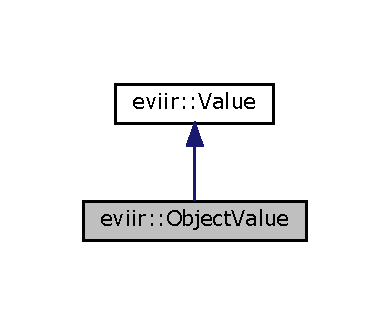
\includegraphics[width=187pt]{classeviir_1_1ObjectValue__inherit__graph}
\end{center}
\end{figure}


Collaboration diagram for eviir\+:\+:Object\+Value\+:\nopagebreak
\begin{figure}[H]
\begin{center}
\leavevmode
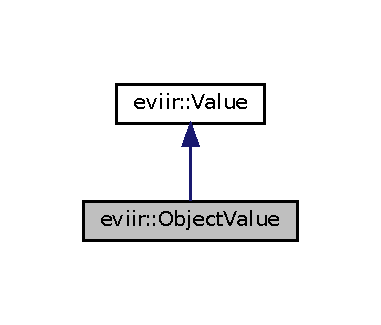
\includegraphics[width=187pt]{classeviir_1_1ObjectValue__coll__graph}
\end{center}
\end{figure}
\subsection*{Public Member Functions}
\begin{DoxyCompactItemize}
\item 
string \hyperlink{classeviir_1_1ObjectValue_a72adc8371c09638a785ed3823516e817}{generate\+\_\+ir} (const char $\ast$format=nullptr)
\item 
\mbox{\Hypertarget{classeviir_1_1ObjectValue_a1a8c705d4f08c5f9be1650188985c79a}\label{classeviir_1_1ObjectValue_a1a8c705d4f08c5f9be1650188985c79a}} 
{\bfseries Object\+Value} (map$<$ \hyperlink{classeviir_1_1Value}{Value} $\ast$C\+O\+M\+MA \hyperlink{classeviir_1_1Value}{Value} $\ast$$>$ pairs)
\end{DoxyCompactItemize}
\subsection*{Public Attributes}
\begin{DoxyCompactItemize}
\item 
\mbox{\Hypertarget{classeviir_1_1ObjectValue_a650b6fad2e883e7e006ce8ca491a94e1}\label{classeviir_1_1ObjectValue_a650b6fad2e883e7e006ce8ca491a94e1}} 
map$<$ \hyperlink{classeviir_1_1Value}{Value} $\ast$C\+O\+M\+MA \hyperlink{classeviir_1_1Value}{Value} $\ast$ $>$ {\bfseries pairs}
\end{DoxyCompactItemize}
\subsection*{Additional Inherited Members}


\subsection{Member Function Documentation}
\mbox{\Hypertarget{classeviir_1_1ObjectValue_a72adc8371c09638a785ed3823516e817}\label{classeviir_1_1ObjectValue_a72adc8371c09638a785ed3823516e817}} 
\index{eviir\+::\+Object\+Value@{eviir\+::\+Object\+Value}!generate\+\_\+ir@{generate\+\_\+ir}}
\index{generate\+\_\+ir@{generate\+\_\+ir}!eviir\+::\+Object\+Value@{eviir\+::\+Object\+Value}}
\subsubsection{\texorpdfstring{generate\+\_\+ir()}{generate\_ir()}}
{\footnotesize\ttfamily string eviir\+::\+Object\+Value\+::generate\+\_\+ir (\begin{DoxyParamCaption}\item[{const char $\ast$}]{format = {\ttfamily nullptr} }\end{DoxyParamCaption})\hspace{0.3cm}{\ttfamily [virtual]}}

Generates the IR for the value \begin{DoxyReturn}{Returns}
the IR as a string (without newline) 
\end{DoxyReturn}


Implements \hyperlink{classeviir_1_1Value_a0613bf660425df31e230681555f64dea}{eviir\+::\+Value}.



The documentation for this class was generated from the following file\+:\begin{DoxyCompactItemize}
\item 
include/ir/value.\+hpp\end{DoxyCompactItemize}

\hypertarget{classeviir_1_1OptionValue}{}\section{eviir\+:\+:Option\+Value Class Reference}
\label{classeviir_1_1OptionValue}\index{eviir\+::\+Option\+Value@{eviir\+::\+Option\+Value}}


Inheritance diagram for eviir\+:\+:Option\+Value\+:\nopagebreak
\begin{figure}[H]
\begin{center}
\leavevmode
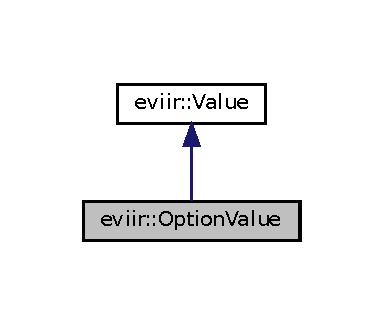
\includegraphics[width=188pt]{classeviir_1_1OptionValue__inherit__graph}
\end{center}
\end{figure}


Collaboration diagram for eviir\+:\+:Option\+Value\+:\nopagebreak
\begin{figure}[H]
\begin{center}
\leavevmode
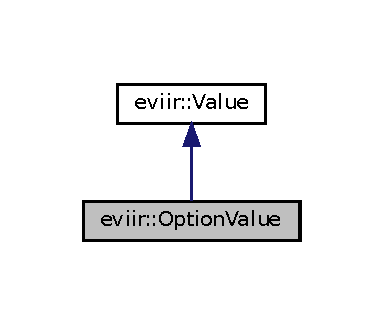
\includegraphics[width=188pt]{classeviir_1_1OptionValue__coll__graph}
\end{center}
\end{figure}
\subsection*{Public Member Functions}
\begin{DoxyCompactItemize}
\item 
string \hyperlink{classeviir_1_1OptionValue_abb9e9cbaa9f6c0af697e5cbea035f56a}{generate\+\_\+ir} (const char $\ast$format=nullptr)
\item 
\mbox{\Hypertarget{classeviir_1_1OptionValue_a471275196d5d4d074a3a0af18ca78210}\label{classeviir_1_1OptionValue_a471275196d5d4d074a3a0af18ca78210}} 
{\bfseries Option\+Value} (string name)
\end{DoxyCompactItemize}
\subsection*{Public Attributes}
\begin{DoxyCompactItemize}
\item 
\mbox{\Hypertarget{classeviir_1_1OptionValue_ab8b3c911a0116a463813ffe5c7cf3c8f}\label{classeviir_1_1OptionValue_ab8b3c911a0116a463813ffe5c7cf3c8f}} 
string {\bfseries name}
\end{DoxyCompactItemize}
\subsection*{Additional Inherited Members}


\subsection{Member Function Documentation}
\mbox{\Hypertarget{classeviir_1_1OptionValue_abb9e9cbaa9f6c0af697e5cbea035f56a}\label{classeviir_1_1OptionValue_abb9e9cbaa9f6c0af697e5cbea035f56a}} 
\index{eviir\+::\+Option\+Value@{eviir\+::\+Option\+Value}!generate\+\_\+ir@{generate\+\_\+ir}}
\index{generate\+\_\+ir@{generate\+\_\+ir}!eviir\+::\+Option\+Value@{eviir\+::\+Option\+Value}}
\subsubsection{\texorpdfstring{generate\+\_\+ir()}{generate\_ir()}}
{\footnotesize\ttfamily string eviir\+::\+Option\+Value\+::generate\+\_\+ir (\begin{DoxyParamCaption}\item[{const char $\ast$}]{format = {\ttfamily nullptr} }\end{DoxyParamCaption})\hspace{0.3cm}{\ttfamily [virtual]}}

Generates the IR for the value \begin{DoxyReturn}{Returns}
the IR as a string (without newline) 
\end{DoxyReturn}


Implements \hyperlink{classeviir_1_1Value_a0613bf660425df31e230681555f64dea}{eviir\+::\+Value}.



The documentation for this class was generated from the following file\+:\begin{DoxyCompactItemize}
\item 
include/ir/value.\+hpp\end{DoxyCompactItemize}

\hypertarget{classeviir_1_1ReferenceValue}{}\doxysection{eviir\+::Reference\+Value Class Reference}
\label{classeviir_1_1ReferenceValue}\index{eviir::ReferenceValue@{eviir::ReferenceValue}}


Inheritance diagram for eviir\+::Reference\+Value\+:\nopagebreak
\begin{figure}[H]
\begin{center}
\leavevmode
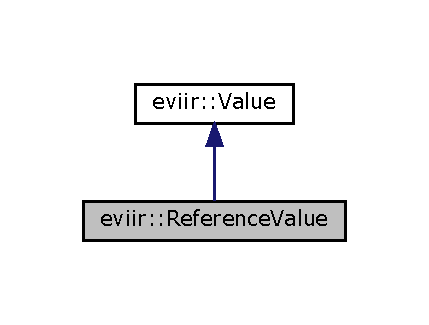
\includegraphics[width=201pt]{classeviir_1_1ReferenceValue__inherit__graph}
\end{center}
\end{figure}


Collaboration diagram for eviir\+::Reference\+Value\+:\nopagebreak
\begin{figure}[H]
\begin{center}
\leavevmode
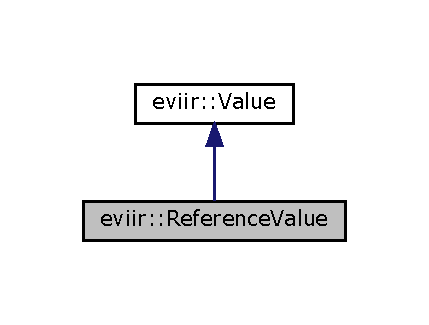
\includegraphics[width=201pt]{classeviir_1_1ReferenceValue__coll__graph}
\end{center}
\end{figure}
\doxysubsection*{Public Member Functions}
\begin{DoxyCompactItemize}
\item 
string \mbox{\hyperlink{classeviir_1_1ReferenceValue_a7b03ad70c7253d44fb7061a91751f9f6}{generate\+\_\+ir}} (const char $\ast$format=nullptr)
\item 
\mbox{\Hypertarget{classeviir_1_1ReferenceValue_ae001aa4a016ccf2a16cd6c0a864a9c20}\label{classeviir_1_1ReferenceValue_ae001aa4a016ccf2a16cd6c0a864a9c20}} 
{\bfseries Reference\+Value} (string name)
\end{DoxyCompactItemize}
\doxysubsection*{Public Attributes}
\begin{DoxyCompactItemize}
\item 
\mbox{\Hypertarget{classeviir_1_1ReferenceValue_a85868eceda63d8196653fee17207a16a}\label{classeviir_1_1ReferenceValue_a85868eceda63d8196653fee17207a16a}} 
string {\bfseries name}
\end{DoxyCompactItemize}
\doxysubsection*{Additional Inherited Members}


\doxysubsection{Member Function Documentation}
\mbox{\Hypertarget{classeviir_1_1ReferenceValue_a7b03ad70c7253d44fb7061a91751f9f6}\label{classeviir_1_1ReferenceValue_a7b03ad70c7253d44fb7061a91751f9f6}} 
\index{eviir::ReferenceValue@{eviir::ReferenceValue}!generate\_ir@{generate\_ir}}
\index{generate\_ir@{generate\_ir}!eviir::ReferenceValue@{eviir::ReferenceValue}}
\doxysubsubsection{\texorpdfstring{generate\_ir()}{generate\_ir()}}
{\footnotesize\ttfamily string eviir\+::\+Reference\+Value\+::generate\+\_\+ir (\begin{DoxyParamCaption}\item[{const char $\ast$}]{format = {\ttfamily nullptr} }\end{DoxyParamCaption})\hspace{0.3cm}{\ttfamily [virtual]}}

Generates the IR for the value \begin{DoxyReturn}{Returns}
the IR as a string (without newline) 
\end{DoxyReturn}


Implements \mbox{\hyperlink{classeviir_1_1Value_a0613bf660425df31e230681555f64dea}{eviir\+::\+Value}}.



The documentation for this class was generated from the following file\+:\begin{DoxyCompactItemize}
\item 
/home/sjoerd/\+Coding/\+Languages/\+Evi\+Ir/include/ir/value.\+hpp\end{DoxyCompactItemize}

\hypertarget{classeviir_1_1StringValue}{}\doxysection{eviir\+::String\+Value Class Reference}
\label{classeviir_1_1StringValue}\index{eviir::StringValue@{eviir::StringValue}}


Inheritance diagram for eviir\+::String\+Value\+:\nopagebreak
\begin{figure}[H]
\begin{center}
\leavevmode
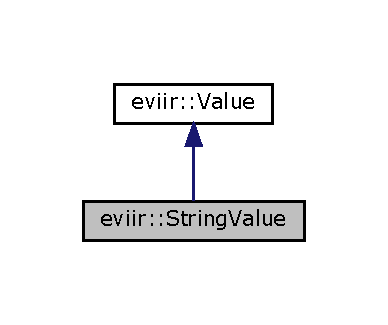
\includegraphics[width=180pt]{classeviir_1_1StringValue__inherit__graph}
\end{center}
\end{figure}


Collaboration diagram for eviir\+::String\+Value\+:\nopagebreak
\begin{figure}[H]
\begin{center}
\leavevmode
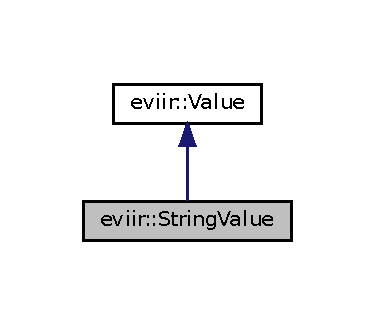
\includegraphics[width=180pt]{classeviir_1_1StringValue__coll__graph}
\end{center}
\end{figure}
\doxysubsection*{Public Member Functions}
\begin{DoxyCompactItemize}
\item 
string \mbox{\hyperlink{classeviir_1_1StringValue_ab8c17f9426e993cd01bd67958aba0038}{generate\+\_\+ir}} (const char $\ast$format=nullptr)
\item 
\mbox{\Hypertarget{classeviir_1_1StringValue_a53a941b534b65d2d0ac1a3737f5cb678}\label{classeviir_1_1StringValue_a53a941b534b65d2d0ac1a3737f5cb678}} 
{\bfseries String\+Value} (string value)
\end{DoxyCompactItemize}
\doxysubsection*{Public Attributes}
\begin{DoxyCompactItemize}
\item 
\mbox{\Hypertarget{classeviir_1_1StringValue_a2dc8191eec0dac183451665d080bcafd}\label{classeviir_1_1StringValue_a2dc8191eec0dac183451665d080bcafd}} 
string {\bfseries value}
\end{DoxyCompactItemize}
\doxysubsection*{Additional Inherited Members}


\doxysubsection{Member Function Documentation}
\mbox{\Hypertarget{classeviir_1_1StringValue_ab8c17f9426e993cd01bd67958aba0038}\label{classeviir_1_1StringValue_ab8c17f9426e993cd01bd67958aba0038}} 
\index{eviir::StringValue@{eviir::StringValue}!generate\_ir@{generate\_ir}}
\index{generate\_ir@{generate\_ir}!eviir::StringValue@{eviir::StringValue}}
\doxysubsubsection{\texorpdfstring{generate\_ir()}{generate\_ir()}}
{\footnotesize\ttfamily string eviir\+::\+String\+Value\+::generate\+\_\+ir (\begin{DoxyParamCaption}\item[{const char $\ast$}]{format = {\ttfamily nullptr} }\end{DoxyParamCaption})\hspace{0.3cm}{\ttfamily [virtual]}}

Generates the IR for the value \begin{DoxyReturn}{Returns}
the IR as a string (without newline) 
\end{DoxyReturn}


Implements \mbox{\hyperlink{classeviir_1_1Value_a0613bf660425df31e230681555f64dea}{eviir\+::\+Value}}.



The documentation for this class was generated from the following file\+:\begin{DoxyCompactItemize}
\item 
/home/sjoerd/\+Coding/\+Languages/\+Evi\+Ir/include/ir/value.\+hpp\end{DoxyCompactItemize}

\hypertarget{classeviir_1_1Value}{}\section{eviir\+:\+:Value Class Reference}
\label{classeviir_1_1Value}\index{eviir\+::\+Value@{eviir\+::\+Value}}


Inheritance diagram for eviir\+:\+:Value\+:\nopagebreak
\begin{figure}[H]
\begin{center}
\leavevmode
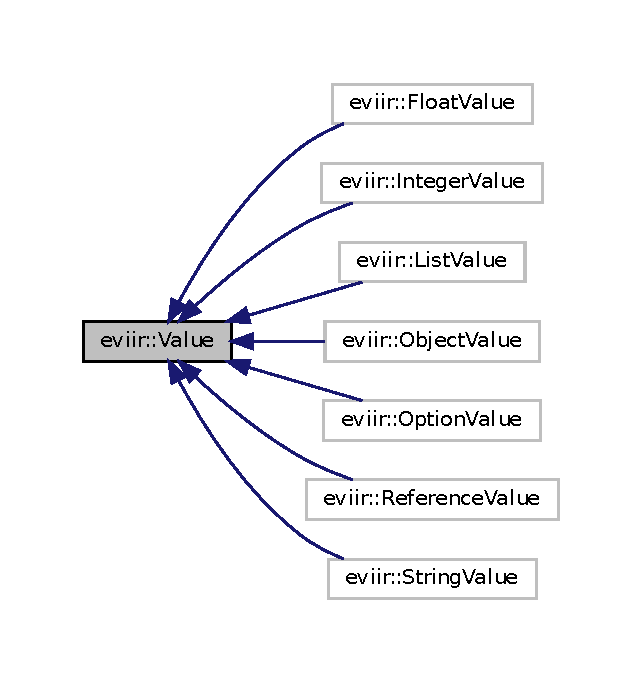
\includegraphics[width=318pt]{classeviir_1_1Value__inherit__graph}
\end{center}
\end{figure}
\subsection*{Public Member Functions}
\begin{DoxyCompactItemize}
\item 
\hyperlink{classeviir_1_1Value_a6870e847f6b19c002b34ad62f2b09da0}{S\+I\+M\+P\+L\+E\+\_\+\+V\+A\+L\+U\+E\+\_\+\+C\+O\+N\+T\+R\+U\+C\+T\+OR} (\hyperlink{classeviir_1_1IntegerValue}{Integer\+Value}, integer, int64, value)
\item 
\hyperlink{classeviir_1_1Value_a3617c67c6a086ea32d6c555a57120003}{S\+I\+M\+P\+L\+E\+\_\+\+V\+A\+L\+U\+E\+\_\+\+C\+O\+N\+T\+R\+U\+C\+T\+OR} (\hyperlink{classeviir_1_1FloatValue}{Float\+Value}, float, float2, value)
\item 
\hyperlink{classeviir_1_1Value_ae1a5aed10e2b2c0a7b76a06a74cf00cf}{S\+I\+M\+P\+L\+E\+\_\+\+V\+A\+L\+U\+E\+\_\+\+C\+O\+N\+T\+R\+U\+C\+T\+OR} (\hyperlink{classeviir_1_1StringValue}{String\+Value}, string, string, value)
\item 
\hyperlink{classeviir_1_1Value_aaa32965c6f0535817b09cacd75b30c67}{S\+I\+M\+P\+L\+E\+\_\+\+V\+A\+L\+U\+E\+\_\+\+C\+O\+N\+T\+R\+U\+C\+T\+OR} (\hyperlink{classeviir_1_1ListValue}{List\+Value}, list, vector$<$ \hyperlink{classeviir_1_1Value}{Value} $\ast$$>$, elements)
\item 
\hyperlink{classeviir_1_1Value_a89848fcdb3d649a6a7f0813c6e38c904}{S\+I\+M\+P\+L\+E\+\_\+\+V\+A\+L\+U\+E\+\_\+\+C\+O\+N\+T\+R\+U\+C\+T\+OR} (\hyperlink{classeviir_1_1ObjectValue}{Object\+Value}, object, map$<$ \hyperlink{classeviir_1_1Value}{Value} $\ast$C\+O\+M\+MA \hyperlink{classeviir_1_1Value}{Value} $\ast$$>$, pairs)
\item 
\hyperlink{classeviir_1_1Value_a2e213dc1ba72a82016c3d8d6f4db4afb}{S\+I\+M\+P\+L\+E\+\_\+\+V\+A\+L\+U\+E\+\_\+\+C\+O\+N\+T\+R\+U\+C\+T\+OR} (\hyperlink{classeviir_1_1ReferenceValue}{Reference\+Value}, reference, string, name)
\item 
\hyperlink{classeviir_1_1Value_ad872325f078f87de60adbeae6eab8f98}{S\+I\+M\+P\+L\+E\+\_\+\+V\+A\+L\+U\+E\+\_\+\+C\+O\+N\+T\+R\+U\+C\+T\+OR} (\hyperlink{classeviir_1_1OptionValue}{Option\+Value}, option, string, name)
\item 
virtual string \hyperlink{classeviir_1_1Value_a0613bf660425df31e230681555f64dea}{generate\+\_\+ir} (const char $\ast$format=nullptr)=0
\end{DoxyCompactItemize}


\subsection{Member Function Documentation}
\mbox{\Hypertarget{classeviir_1_1Value_a0613bf660425df31e230681555f64dea}\label{classeviir_1_1Value_a0613bf660425df31e230681555f64dea}} 
\index{eviir\+::\+Value@{eviir\+::\+Value}!generate\+\_\+ir@{generate\+\_\+ir}}
\index{generate\+\_\+ir@{generate\+\_\+ir}!eviir\+::\+Value@{eviir\+::\+Value}}
\subsubsection{\texorpdfstring{generate\+\_\+ir()}{generate\_ir()}}
{\footnotesize\ttfamily virtual string eviir\+::\+Value\+::generate\+\_\+ir (\begin{DoxyParamCaption}\item[{const char $\ast$}]{format = {\ttfamily nullptr} }\end{DoxyParamCaption})\hspace{0.3cm}{\ttfamily [pure virtual]}}

Generates the IR for the value \begin{DoxyReturn}{Returns}
the IR as a string (without newline) 
\end{DoxyReturn}


Implemented in \hyperlink{classeviir_1_1OptionValue_abb9e9cbaa9f6c0af697e5cbea035f56a}{eviir\+::\+Option\+Value}, \hyperlink{classeviir_1_1ReferenceValue_a7b03ad70c7253d44fb7061a91751f9f6}{eviir\+::\+Reference\+Value}, \hyperlink{classeviir_1_1ObjectValue_a72adc8371c09638a785ed3823516e817}{eviir\+::\+Object\+Value}, \hyperlink{classeviir_1_1ListValue_ad12dee3774ad443ad0e27354909e8dc9}{eviir\+::\+List\+Value}, \hyperlink{classeviir_1_1StringValue_ab8c17f9426e993cd01bd67958aba0038}{eviir\+::\+String\+Value}, \hyperlink{classeviir_1_1FloatValue_a8713d6eb43445ba56c4104bce8fe7070}{eviir\+::\+Float\+Value}, and \hyperlink{classeviir_1_1IntegerValue_a7f2653e23a8165a0eb43109d152cc0a2}{eviir\+::\+Integer\+Value}.

\mbox{\Hypertarget{classeviir_1_1Value_a6870e847f6b19c002b34ad62f2b09da0}\label{classeviir_1_1Value_a6870e847f6b19c002b34ad62f2b09da0}} 
\index{eviir\+::\+Value@{eviir\+::\+Value}!S\+I\+M\+P\+L\+E\+\_\+\+V\+A\+L\+U\+E\+\_\+\+C\+O\+N\+T\+R\+U\+C\+T\+OR@{S\+I\+M\+P\+L\+E\+\_\+\+V\+A\+L\+U\+E\+\_\+\+C\+O\+N\+T\+R\+U\+C\+T\+OR}}
\index{S\+I\+M\+P\+L\+E\+\_\+\+V\+A\+L\+U\+E\+\_\+\+C\+O\+N\+T\+R\+U\+C\+T\+OR@{S\+I\+M\+P\+L\+E\+\_\+\+V\+A\+L\+U\+E\+\_\+\+C\+O\+N\+T\+R\+U\+C\+T\+OR}!eviir\+::\+Value@{eviir\+::\+Value}}
\subsubsection{\texorpdfstring{S\+I\+M\+P\+L\+E\+\_\+\+V\+A\+L\+U\+E\+\_\+\+C\+O\+N\+T\+R\+U\+C\+T\+O\+R()}{SIMPLE\_VALUE\_CONTRUCTOR()}\hspace{0.1cm}{\footnotesize\ttfamily [1/7]}}
{\footnotesize\ttfamily eviir\+::\+Value\+::\+S\+I\+M\+P\+L\+E\+\_\+\+V\+A\+L\+U\+E\+\_\+\+C\+O\+N\+T\+R\+U\+C\+T\+OR (\begin{DoxyParamCaption}\item[{\hyperlink{classeviir_1_1IntegerValue}{Integer\+Value}}]{,  }\item[{integer}]{,  }\item[{int64}]{,  }\item[{value}]{ }\end{DoxyParamCaption})}

Constructs a new integer value 
\begin{DoxyParams}{Parameters}
{\em value} & the integer \\
\hline
\end{DoxyParams}
\mbox{\Hypertarget{classeviir_1_1Value_a3617c67c6a086ea32d6c555a57120003}\label{classeviir_1_1Value_a3617c67c6a086ea32d6c555a57120003}} 
\index{eviir\+::\+Value@{eviir\+::\+Value}!S\+I\+M\+P\+L\+E\+\_\+\+V\+A\+L\+U\+E\+\_\+\+C\+O\+N\+T\+R\+U\+C\+T\+OR@{S\+I\+M\+P\+L\+E\+\_\+\+V\+A\+L\+U\+E\+\_\+\+C\+O\+N\+T\+R\+U\+C\+T\+OR}}
\index{S\+I\+M\+P\+L\+E\+\_\+\+V\+A\+L\+U\+E\+\_\+\+C\+O\+N\+T\+R\+U\+C\+T\+OR@{S\+I\+M\+P\+L\+E\+\_\+\+V\+A\+L\+U\+E\+\_\+\+C\+O\+N\+T\+R\+U\+C\+T\+OR}!eviir\+::\+Value@{eviir\+::\+Value}}
\subsubsection{\texorpdfstring{S\+I\+M\+P\+L\+E\+\_\+\+V\+A\+L\+U\+E\+\_\+\+C\+O\+N\+T\+R\+U\+C\+T\+O\+R()}{SIMPLE\_VALUE\_CONTRUCTOR()}\hspace{0.1cm}{\footnotesize\ttfamily [2/7]}}
{\footnotesize\ttfamily eviir\+::\+Value\+::\+S\+I\+M\+P\+L\+E\+\_\+\+V\+A\+L\+U\+E\+\_\+\+C\+O\+N\+T\+R\+U\+C\+T\+OR (\begin{DoxyParamCaption}\item[{\hyperlink{classeviir_1_1FloatValue}{Float\+Value}}]{,  }\item[{float}]{,  }\item[{float2}]{,  }\item[{value}]{ }\end{DoxyParamCaption})}

Constructs a new float value 
\begin{DoxyParams}{Parameters}
{\em value} & the float \\
\hline
\end{DoxyParams}
\mbox{\Hypertarget{classeviir_1_1Value_ae1a5aed10e2b2c0a7b76a06a74cf00cf}\label{classeviir_1_1Value_ae1a5aed10e2b2c0a7b76a06a74cf00cf}} 
\index{eviir\+::\+Value@{eviir\+::\+Value}!S\+I\+M\+P\+L\+E\+\_\+\+V\+A\+L\+U\+E\+\_\+\+C\+O\+N\+T\+R\+U\+C\+T\+OR@{S\+I\+M\+P\+L\+E\+\_\+\+V\+A\+L\+U\+E\+\_\+\+C\+O\+N\+T\+R\+U\+C\+T\+OR}}
\index{S\+I\+M\+P\+L\+E\+\_\+\+V\+A\+L\+U\+E\+\_\+\+C\+O\+N\+T\+R\+U\+C\+T\+OR@{S\+I\+M\+P\+L\+E\+\_\+\+V\+A\+L\+U\+E\+\_\+\+C\+O\+N\+T\+R\+U\+C\+T\+OR}!eviir\+::\+Value@{eviir\+::\+Value}}
\subsubsection{\texorpdfstring{S\+I\+M\+P\+L\+E\+\_\+\+V\+A\+L\+U\+E\+\_\+\+C\+O\+N\+T\+R\+U\+C\+T\+O\+R()}{SIMPLE\_VALUE\_CONTRUCTOR()}\hspace{0.1cm}{\footnotesize\ttfamily [3/7]}}
{\footnotesize\ttfamily eviir\+::\+Value\+::\+S\+I\+M\+P\+L\+E\+\_\+\+V\+A\+L\+U\+E\+\_\+\+C\+O\+N\+T\+R\+U\+C\+T\+OR (\begin{DoxyParamCaption}\item[{\hyperlink{classeviir_1_1StringValue}{String\+Value}}]{,  }\item[{string}]{,  }\item[{string}]{,  }\item[{value}]{ }\end{DoxyParamCaption})}

Constructs a new string value 
\begin{DoxyParams}{Parameters}
{\em value} & the string \\
\hline
\end{DoxyParams}
\mbox{\Hypertarget{classeviir_1_1Value_aaa32965c6f0535817b09cacd75b30c67}\label{classeviir_1_1Value_aaa32965c6f0535817b09cacd75b30c67}} 
\index{eviir\+::\+Value@{eviir\+::\+Value}!S\+I\+M\+P\+L\+E\+\_\+\+V\+A\+L\+U\+E\+\_\+\+C\+O\+N\+T\+R\+U\+C\+T\+OR@{S\+I\+M\+P\+L\+E\+\_\+\+V\+A\+L\+U\+E\+\_\+\+C\+O\+N\+T\+R\+U\+C\+T\+OR}}
\index{S\+I\+M\+P\+L\+E\+\_\+\+V\+A\+L\+U\+E\+\_\+\+C\+O\+N\+T\+R\+U\+C\+T\+OR@{S\+I\+M\+P\+L\+E\+\_\+\+V\+A\+L\+U\+E\+\_\+\+C\+O\+N\+T\+R\+U\+C\+T\+OR}!eviir\+::\+Value@{eviir\+::\+Value}}
\subsubsection{\texorpdfstring{S\+I\+M\+P\+L\+E\+\_\+\+V\+A\+L\+U\+E\+\_\+\+C\+O\+N\+T\+R\+U\+C\+T\+O\+R()}{SIMPLE\_VALUE\_CONTRUCTOR()}\hspace{0.1cm}{\footnotesize\ttfamily [4/7]}}
{\footnotesize\ttfamily eviir\+::\+Value\+::\+S\+I\+M\+P\+L\+E\+\_\+\+V\+A\+L\+U\+E\+\_\+\+C\+O\+N\+T\+R\+U\+C\+T\+OR (\begin{DoxyParamCaption}\item[{\hyperlink{classeviir_1_1ListValue}{List\+Value}}]{,  }\item[{list}]{,  }\item[{vector$<$ \hyperlink{classeviir_1_1Value}{Value} $\ast$$>$}]{,  }\item[{elements}]{ }\end{DoxyParamCaption})}

Constructs a new list value 
\begin{DoxyParams}{Parameters}
{\em elements} & the elements of the list \\
\hline
\end{DoxyParams}
\mbox{\Hypertarget{classeviir_1_1Value_a89848fcdb3d649a6a7f0813c6e38c904}\label{classeviir_1_1Value_a89848fcdb3d649a6a7f0813c6e38c904}} 
\index{eviir\+::\+Value@{eviir\+::\+Value}!S\+I\+M\+P\+L\+E\+\_\+\+V\+A\+L\+U\+E\+\_\+\+C\+O\+N\+T\+R\+U\+C\+T\+OR@{S\+I\+M\+P\+L\+E\+\_\+\+V\+A\+L\+U\+E\+\_\+\+C\+O\+N\+T\+R\+U\+C\+T\+OR}}
\index{S\+I\+M\+P\+L\+E\+\_\+\+V\+A\+L\+U\+E\+\_\+\+C\+O\+N\+T\+R\+U\+C\+T\+OR@{S\+I\+M\+P\+L\+E\+\_\+\+V\+A\+L\+U\+E\+\_\+\+C\+O\+N\+T\+R\+U\+C\+T\+OR}!eviir\+::\+Value@{eviir\+::\+Value}}
\subsubsection{\texorpdfstring{S\+I\+M\+P\+L\+E\+\_\+\+V\+A\+L\+U\+E\+\_\+\+C\+O\+N\+T\+R\+U\+C\+T\+O\+R()}{SIMPLE\_VALUE\_CONTRUCTOR()}\hspace{0.1cm}{\footnotesize\ttfamily [5/7]}}
{\footnotesize\ttfamily eviir\+::\+Value\+::\+S\+I\+M\+P\+L\+E\+\_\+\+V\+A\+L\+U\+E\+\_\+\+C\+O\+N\+T\+R\+U\+C\+T\+OR (\begin{DoxyParamCaption}\item[{\hyperlink{classeviir_1_1ObjectValue}{Object\+Value}}]{,  }\item[{object}]{,  }\item[{map$<$ \hyperlink{classeviir_1_1Value}{Value} $\ast$C\+O\+M\+MA \hyperlink{classeviir_1_1Value}{Value} $\ast$$>$}]{,  }\item[{pairs}]{ }\end{DoxyParamCaption})}

Constructs a new object value 
\begin{DoxyParams}{Parameters}
{\em pair} & the key-\/value pairs of the object \\
\hline
\end{DoxyParams}
\mbox{\Hypertarget{classeviir_1_1Value_a2e213dc1ba72a82016c3d8d6f4db4afb}\label{classeviir_1_1Value_a2e213dc1ba72a82016c3d8d6f4db4afb}} 
\index{eviir\+::\+Value@{eviir\+::\+Value}!S\+I\+M\+P\+L\+E\+\_\+\+V\+A\+L\+U\+E\+\_\+\+C\+O\+N\+T\+R\+U\+C\+T\+OR@{S\+I\+M\+P\+L\+E\+\_\+\+V\+A\+L\+U\+E\+\_\+\+C\+O\+N\+T\+R\+U\+C\+T\+OR}}
\index{S\+I\+M\+P\+L\+E\+\_\+\+V\+A\+L\+U\+E\+\_\+\+C\+O\+N\+T\+R\+U\+C\+T\+OR@{S\+I\+M\+P\+L\+E\+\_\+\+V\+A\+L\+U\+E\+\_\+\+C\+O\+N\+T\+R\+U\+C\+T\+OR}!eviir\+::\+Value@{eviir\+::\+Value}}
\subsubsection{\texorpdfstring{S\+I\+M\+P\+L\+E\+\_\+\+V\+A\+L\+U\+E\+\_\+\+C\+O\+N\+T\+R\+U\+C\+T\+O\+R()}{SIMPLE\_VALUE\_CONTRUCTOR()}\hspace{0.1cm}{\footnotesize\ttfamily [6/7]}}
{\footnotesize\ttfamily eviir\+::\+Value\+::\+S\+I\+M\+P\+L\+E\+\_\+\+V\+A\+L\+U\+E\+\_\+\+C\+O\+N\+T\+R\+U\+C\+T\+OR (\begin{DoxyParamCaption}\item[{\hyperlink{classeviir_1_1ReferenceValue}{Reference\+Value}}]{,  }\item[{reference}]{,  }\item[{string}]{,  }\item[{name}]{ }\end{DoxyParamCaption})}

Constructs a new reference value 
\begin{DoxyParams}{Parameters}
{\em name} & the name of the reference \\
\hline
\end{DoxyParams}
\mbox{\Hypertarget{classeviir_1_1Value_ad872325f078f87de60adbeae6eab8f98}\label{classeviir_1_1Value_ad872325f078f87de60adbeae6eab8f98}} 
\index{eviir\+::\+Value@{eviir\+::\+Value}!S\+I\+M\+P\+L\+E\+\_\+\+V\+A\+L\+U\+E\+\_\+\+C\+O\+N\+T\+R\+U\+C\+T\+OR@{S\+I\+M\+P\+L\+E\+\_\+\+V\+A\+L\+U\+E\+\_\+\+C\+O\+N\+T\+R\+U\+C\+T\+OR}}
\index{S\+I\+M\+P\+L\+E\+\_\+\+V\+A\+L\+U\+E\+\_\+\+C\+O\+N\+T\+R\+U\+C\+T\+OR@{S\+I\+M\+P\+L\+E\+\_\+\+V\+A\+L\+U\+E\+\_\+\+C\+O\+N\+T\+R\+U\+C\+T\+OR}!eviir\+::\+Value@{eviir\+::\+Value}}
\subsubsection{\texorpdfstring{S\+I\+M\+P\+L\+E\+\_\+\+V\+A\+L\+U\+E\+\_\+\+C\+O\+N\+T\+R\+U\+C\+T\+O\+R()}{SIMPLE\_VALUE\_CONTRUCTOR()}\hspace{0.1cm}{\footnotesize\ttfamily [7/7]}}
{\footnotesize\ttfamily eviir\+::\+Value\+::\+S\+I\+M\+P\+L\+E\+\_\+\+V\+A\+L\+U\+E\+\_\+\+C\+O\+N\+T\+R\+U\+C\+T\+OR (\begin{DoxyParamCaption}\item[{\hyperlink{classeviir_1_1OptionValue}{Option\+Value}}]{,  }\item[{option}]{,  }\item[{string}]{,  }\item[{name}]{ }\end{DoxyParamCaption})}

Constructs a new option value 
\begin{DoxyParams}{Parameters}
{\em name} & the name of the option \\
\hline
\end{DoxyParams}


The documentation for this class was generated from the following file\+:\begin{DoxyCompactItemize}
\item 
include/ir/value.\+hpp\end{DoxyCompactItemize}

%--- End generated contents ---

% Index
\backmatter
\newpage
\phantomsection
\clearemptydoublepage
\addcontentsline{toc}{chapter}{Index}
\printindex

\end{document}
